\documentclass[aspectratio=169,11pt]{beamer}

\usepackage{tuke-presentation}
\newcommand{\CourseTitle}{Mikroprocesorov\'a technika}
\newcommand{\CourseAuthor}{prof. Ing. Ivan Virgala, PhD.}
\newcommand{\CourseInstitute}{Technick\'a univerzita v Ko\v{s}iciach}
\newcommand{\CourseYear}{Strojn\'icka fakulta}

\graphicspath{{figures/p01/}{figures/common/}}

\title{\CourseTitle}
\subtitle{Prednáška č.1: História a vznik mikrokontrolérov}
\author{\CourseAuthor}
\institute{\CourseInstitute\\Strojnícka fakulta}
\date{Katedra priemyselnej automatizácie a mechatroniky}

\newcommand{\Milestone}[4]{%
\begin{tikzpicture}[baseline]
  \node[draw=MainBlue,fill=#1,rounded corners=2pt,inner sep=5pt,text width=#2,align=center] {\textbf{#3}\\[-1pt]\scriptsize #4};
\end{tikzpicture}%
}
\usepackage{graphicx}
\usepackage{fontawesome5}
\usepackage{tikz}
\usetikzlibrary{shadows}
\newenvironment{definitionbox}[1]
{
\begin{tcolorbox}[
    colback=blue!4,
    colframe=MainBlue,
    rounded corners,
    title={\faLightbulb\quad #1}
]
}
{
\end{tcolorbox}
}
\begin{document}

\TUKEtitleframe

\begin{frame}{Obsah prednášok a cvičení}
\scriptsize
\begin{tabular}{p{0.06\textwidth}p{0.38\textwidth}p{0.46\textwidth}}
\toprule
Týždeň & Prednáška & Cvičenie \\
\midrule
1 & História a vznik mikrokontrolérov & Číselné sústavy, VS Code, UNO R3 \\
2 & ATmega328P a digitálne I/O & LED, tlačidlo, \texttt{DDRx}, \texttt{PORTx}, \texttt{PINx} \\
3 & architektúra a pamäte & bitové masky, stavový automat \\
4 & prerušenia & tlačidlo, inkrementálny enkodér \\
5 & časovače a čítače & časová základňa, meranie frekvencie \\
6 & PWM a DC motor & otvorené riadenie rýchlosti \\
7 & PID/PSD regulácia DC motora & uzavretá slučka s enkodérom \\
8 & servopohony & RC servo alebo DC servopohon \\
9 & krokové motory & STEP/DIR, rampový profil \\
10 & ADC a snímače & meranie, filtrovanie, kalibrácia \\
11 & USART & diagnostika a príkazy \\
12 & SPI a TWI/I$^2$C & nízkoúrovňový ovládač periférie \\
13 & integrácia a spoľahlivosť & záverečná integrovaná úloha \\
\bottomrule
\end{tabular}
\end{frame}

% \begin{frame}{Prečo začíname históriou}
% \begin{columns}[T,onlytextwidth]
% \column{0.56\textwidth}
% \BlueBox{Cieľ nie je memorovať dátumy}{
% História má ukázať, \textbf{prečo} vznikol mikrokontrolér: ako odpoveď na potrebu lacného, spoľahlivého a programovateľného riadenia technických zariadení.
% }
% \vspace{0.15cm}
% \begin{itemize}
%   \item zmena od pevne zapojenej logiky k programu,
%   \item miniaturizácia od elektrónok k integrovaným obvodom,
%   \item integrácia CPU, pamäte a periférií na jeden čip,
%   \item vznik embedded systémov ako samostatnej technickej oblasti.
% \end{itemize}
% \column{0.39\textwidth}
% \begin{alertblock}{Hlavná veta}
% Mikrokontrolér je výsledkom snahy preniesť riadenie z káblov a mechaniky do programu, ale stále ostáva pevne spojený s reálnym hardvérom.
% \end{alertblock}
% \end{columns}
% \end{frame}

\begin{frame}{Čo má študent po prednáške vedieť?}
\begin{itemize}
  \item Vysvetliť rozdiel medzi mikroprocesorom, mikrokontrolérom a embedded systémom,
  \item Zaradiť hlavné historické míľniky: elektrónky, tranzistor, IC, Intel 4004, 8008, 8080, TMS1000, 8086, 8051, AVR,
  \item Pochopiť, prečo je pri mikrokontroléri rozhodujúca integrácia periférií,
  \item Rozumieť, prečo budeme pracovať priamo s registrami ATmega328P,
  \item Vedieť, prečo Arduino UNO R3 používame ako vývojovú dosku, nie ako Arduino framework.
\end{itemize}
\end{frame}

\begin{frame}{Predmet nie je hobby kurz Arduino}
\begin{columns}[T,onlytextwidth]
\column{0.48\textwidth}
\BlueBox{Používame}{
\begin{itemize}
  \item Arduino UNO R3 ako spoľahlivú dosku,
  \item ATmega328P ako cieľový mikrokontrolér,
  \item VS Code, PlatformIO, AVR-GCC, AVR-LibC,
  \item jazyk C a vlastný \texttt{main()}.
\end{itemize}}
\column{0.48\textwidth}
\BlueBox{Nepoužívame}{
\begin{itemize}
  \item \texttt{setup()}, \texttt{loop()}, \texttt{.ino},
  \item \texttt{digitalWrite()}, \texttt{analogRead()}, \texttt{delay()},
  \item hotové knižnice ako náhradu porozumenia,
  \item periférie ako čiernu skrinku.
\end{itemize}}
\end{columns}
\end{frame}



\begin{frame}{Vnorené systémy (embedded systems) v mechatronike}

\begin{columns}[T,onlytextwidth]

% Ľavý stĺpec
\column{0.54\textwidth}

\BlueBox{
    \faIcon[regular]{lightbulb}\hspace{0.5em}Definícia
}{
    Vnorený systém je počítačový systém zabudovaný do väčšieho
    technického zariadenia, ktorý vykonáva konkrétnu meraciu,
    riadiacu, komunikačnú alebo bezpečnostnú funkciu.
}

\vspace{0.15cm}

\begin{itemize}
    \item nie je to univerzálny osobný počítač
    \item pracuje s fyzikálnymi veličinami
    \item často pracuje v reálnom čase
    \item musí reagovať spoľahlivo aj pri poruche
\end{itemize}

% Pravý stĺpec
\column{0.41\textwidth}

\centering
\vspace{0.55cm}

\begin{tikzpicture}
\node[
    inner sep=3pt,
    fill=white,
    draw=MainBlue!35,
    line width=0.6pt,
    rounded corners=6pt,
    drop shadow
]{
    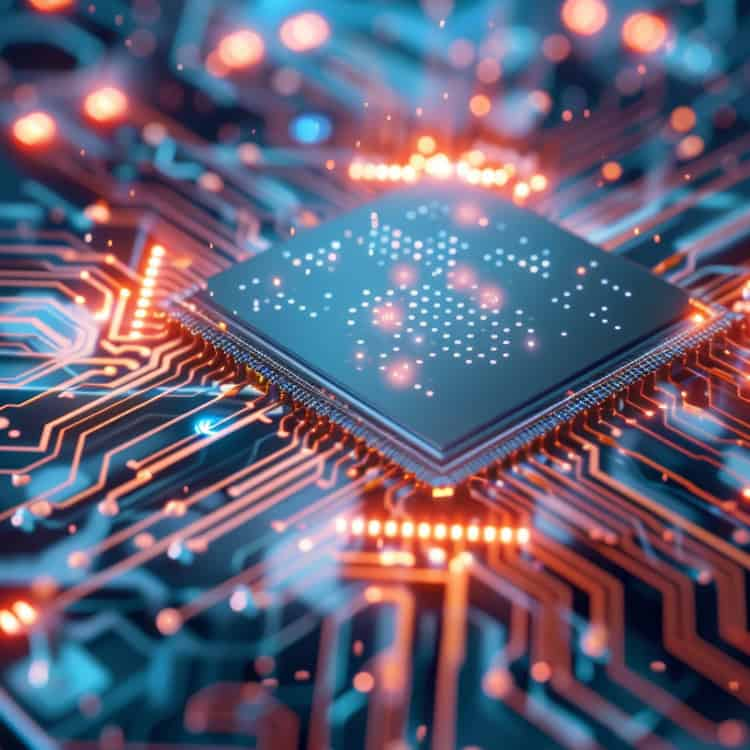
\includegraphics[
        width=0.95\linewidth,
        height=0.60\textheight,
        keepaspectratio
    ]{figures/p01/embedded-systems-an-optimal-alliance-between-hardware-and-software.jpeg}
};
\end{tikzpicture}

\end{columns}

\end{frame}

% ============================================================
% MOTIVÁCIA 1
% ============================================================

\begin{frame}{Prečo sa zaoberať mikroprocesorovou technikou?}

\begin{columns}[T,onlytextwidth]

% Ľavý stĺpec
\column{0.52\textwidth}

\BlueBox{
    \faIcon{microchip}\hspace{0.5em}Základná myšlienka
}{
    Mikrokontrolér prepája algoritmus so skutočným fyzikálnym svetom.
    Meria, rozhoduje a prostredníctvom aktuátorov ovplyvňuje správanie
    technického systému.
}

\vspace{0.15cm}

\begin{itemize}
    \item spracúva údaje zo snímačov,
    \item vykonáva riadiaci algoritmus,
    \item ovláda pohony, ventily, svetlá alebo displeje,
    \item komunikuje s ďalšími zariadeniami,
    \item zabezpečuje diagnostiku a bezpečné správanie.
\end{itemize}

\vspace{0.15cm}

{\small
Na rozdiel od bežného počítača musí vnorený systém často reagovať
v presne stanovenom čase a s obmedzenou pamäťou, výkonom aj spotrebou.
}

% Pravý stĺpec
\column{0.43\textwidth}
\centering
\vspace{0.15cm}
\begin{tikzpicture}[x=1cm,y=1cm]
\node[
    draw=MainBlue,
    fill=LightBlue,
    rounded corners=4pt,
    minimum width=3.8cm,
    minimum height=0.85cm,
    align=center
] (sensor) at (0,2.8)
{\textbf{Snímače}\\[1mm]\scriptsize poloha, teplota, tlak, prúd, ...};

\node[
    draw=MainBlue,
    fill=MainBlue,
    text=white,
    rounded corners=4pt,
    minimum width=3.8cm,
    minimum height=1.05cm,
    align=center
] (mcu) at (0,1.25)
{\textbf{Mikrokontrolér}\\[1mm]\scriptsize meranie, výpočet, rozhodovanie};

\node[
    draw=MainBlue,
    fill=LightBlue,
    rounded corners=4pt,
    minimum width=3.8cm,
    minimum height=0.85cm,
    align=center
] (actuator) at (0,-0.35)
{\textbf{Aktuátory}\\[1mm]\scriptsize motor, ventil, relé, displej};

\node[
    draw=MainBlue,
    fill=TUKEgray,
    rounded corners=4pt,
    minimum width=3.8cm,
    minimum height=0.85cm,
    align=center
] (process) at (0,-1.85)
{\textbf{Fyzikálny proces}\\[1mm]\scriptsize robot, stroj, vozidlo, budova};

\draw[
    ->,
    MainBlue,
    line width=1.1pt
] (sensor) -- (mcu);

\draw[
    ->,
    MainBlue,
    line width=1.1pt
] (mcu) -- (actuator);

\draw[
    ->,
    MainBlue,
    line width=1.1pt
] (actuator) -- (process);

\draw[
    ->,
    MainBlue,
    line width=1.1pt,
    rounded corners=5pt
]
(process.west)
-- ++(-0.45,0)
-- ++(0,4.65)
-- (sensor.west);

\end{tikzpicture}
\end{columns}
\end{frame}

% ============================================================
% MOTIVÁCIA 2
% ============================================================

\begin{frame}{Mikrokontroléry sú ukryté takmer všade}

% ============================================================
% PRVÝ RIADOK
% ============================================================
\begin{columns}[T,onlytextwidth]

\column{0.31\textwidth}

\BlueBox{
    \strut\faIcon{robot}\hspace{0.4em}Robotika
}{
    \parbox[t][1.45cm][t]{\linewidth}{
        Riadenie pohonov, spracovanie snímačov,
        komunikácia a bezpečnostné funkcie.
    }
}

\column{0.31\textwidth}

\BlueBox{
    \strut\faIcon{car}\hspace{0.4em}Automobily
}{
    \parbox[t][1.45cm][t]{\linewidth}{
        Motor, brzdy, airbag, osvetlenie,
        komfortné systémy a asistenčné funkcie.
    }
}

\column{0.31\textwidth}

\BlueBox{
    \strut\faIcon{heartbeat}\hspace{0.4em}Medicína
}{
    \parbox[t][1.45cm][t]{\linewidth}{
        Diagnostické zariadenia, dávkovanie liekov,
        monitorovanie a protetika.
    }
}

\end{columns}

\vspace{0.22cm}

% ============================================================
% DRUHÝ RIADOK
% ============================================================
\begin{columns}[T,onlytextwidth]

\column{0.31\textwidth}

\BlueBox{
    \strut\faIcon{industry}\hspace{0.4em}Priemysel
}{
    \parbox[t][1.45cm][t]{\linewidth}{
        Výrobné stroje, regulátory, meniče,
        snímače a distribuované riadenie.
    }
}

\column{0.31\textwidth}

\BlueBox{
    \strut\faIcon{home}\hspace{0.4em}Budovy
}{
    \parbox[t][1.45cm][t]{\linewidth}{
        Vykurovanie, klimatizácia, zabezpečenie,
        meranie spotreby a automatizácia.
    }
}

\column{0.31\textwidth}

\BlueBox{
    \strut\faIcon{wifi}\hspace{0.4em}Komunikácia
}{
    \parbox[t][1.45cm][t]{\linewidth}{
        Prenos údajov, bezdrôtové siete,
        IoT zariadenia a vzdialená diagnostika.
    }
}

\end{columns}

\vspace{0.28cm}

% \begin{center}
% \begin{minipage}{0.88\textwidth}
%     \centering
%     \small
%     Používateľ často mikrokontrolér ani nevidí. Napriek tomu rozhoduje
%     o funkčnosti, presnosti, spotrebe, spoľahlivosti a bezpečnosti
%     celého zariadenia.
% \end{minipage}
% \end{center}

\end{frame}

% ============================================================
% Vyuzitie
% ============================================================
\begin{frame}{Využitie mikrokontrolérov v praxi}

\centering
\vspace{-0.10cm}

\begin{tikzpicture}[x=1cm,y=1cm]

% Pevná plocha obrázkovej koláže
% Zabraňuje posúvaniu alebo presahovaniu obrázkov.
\path[use as bounding box]
    (-0.2,-0.80) rectangle (13.6,4.85);

% ============================================================
% HORNÝ RIADOK
% ============================================================

% Práčka / domáci spotrebič
\node[inner sep=0pt] at (1.45,3.55) {
    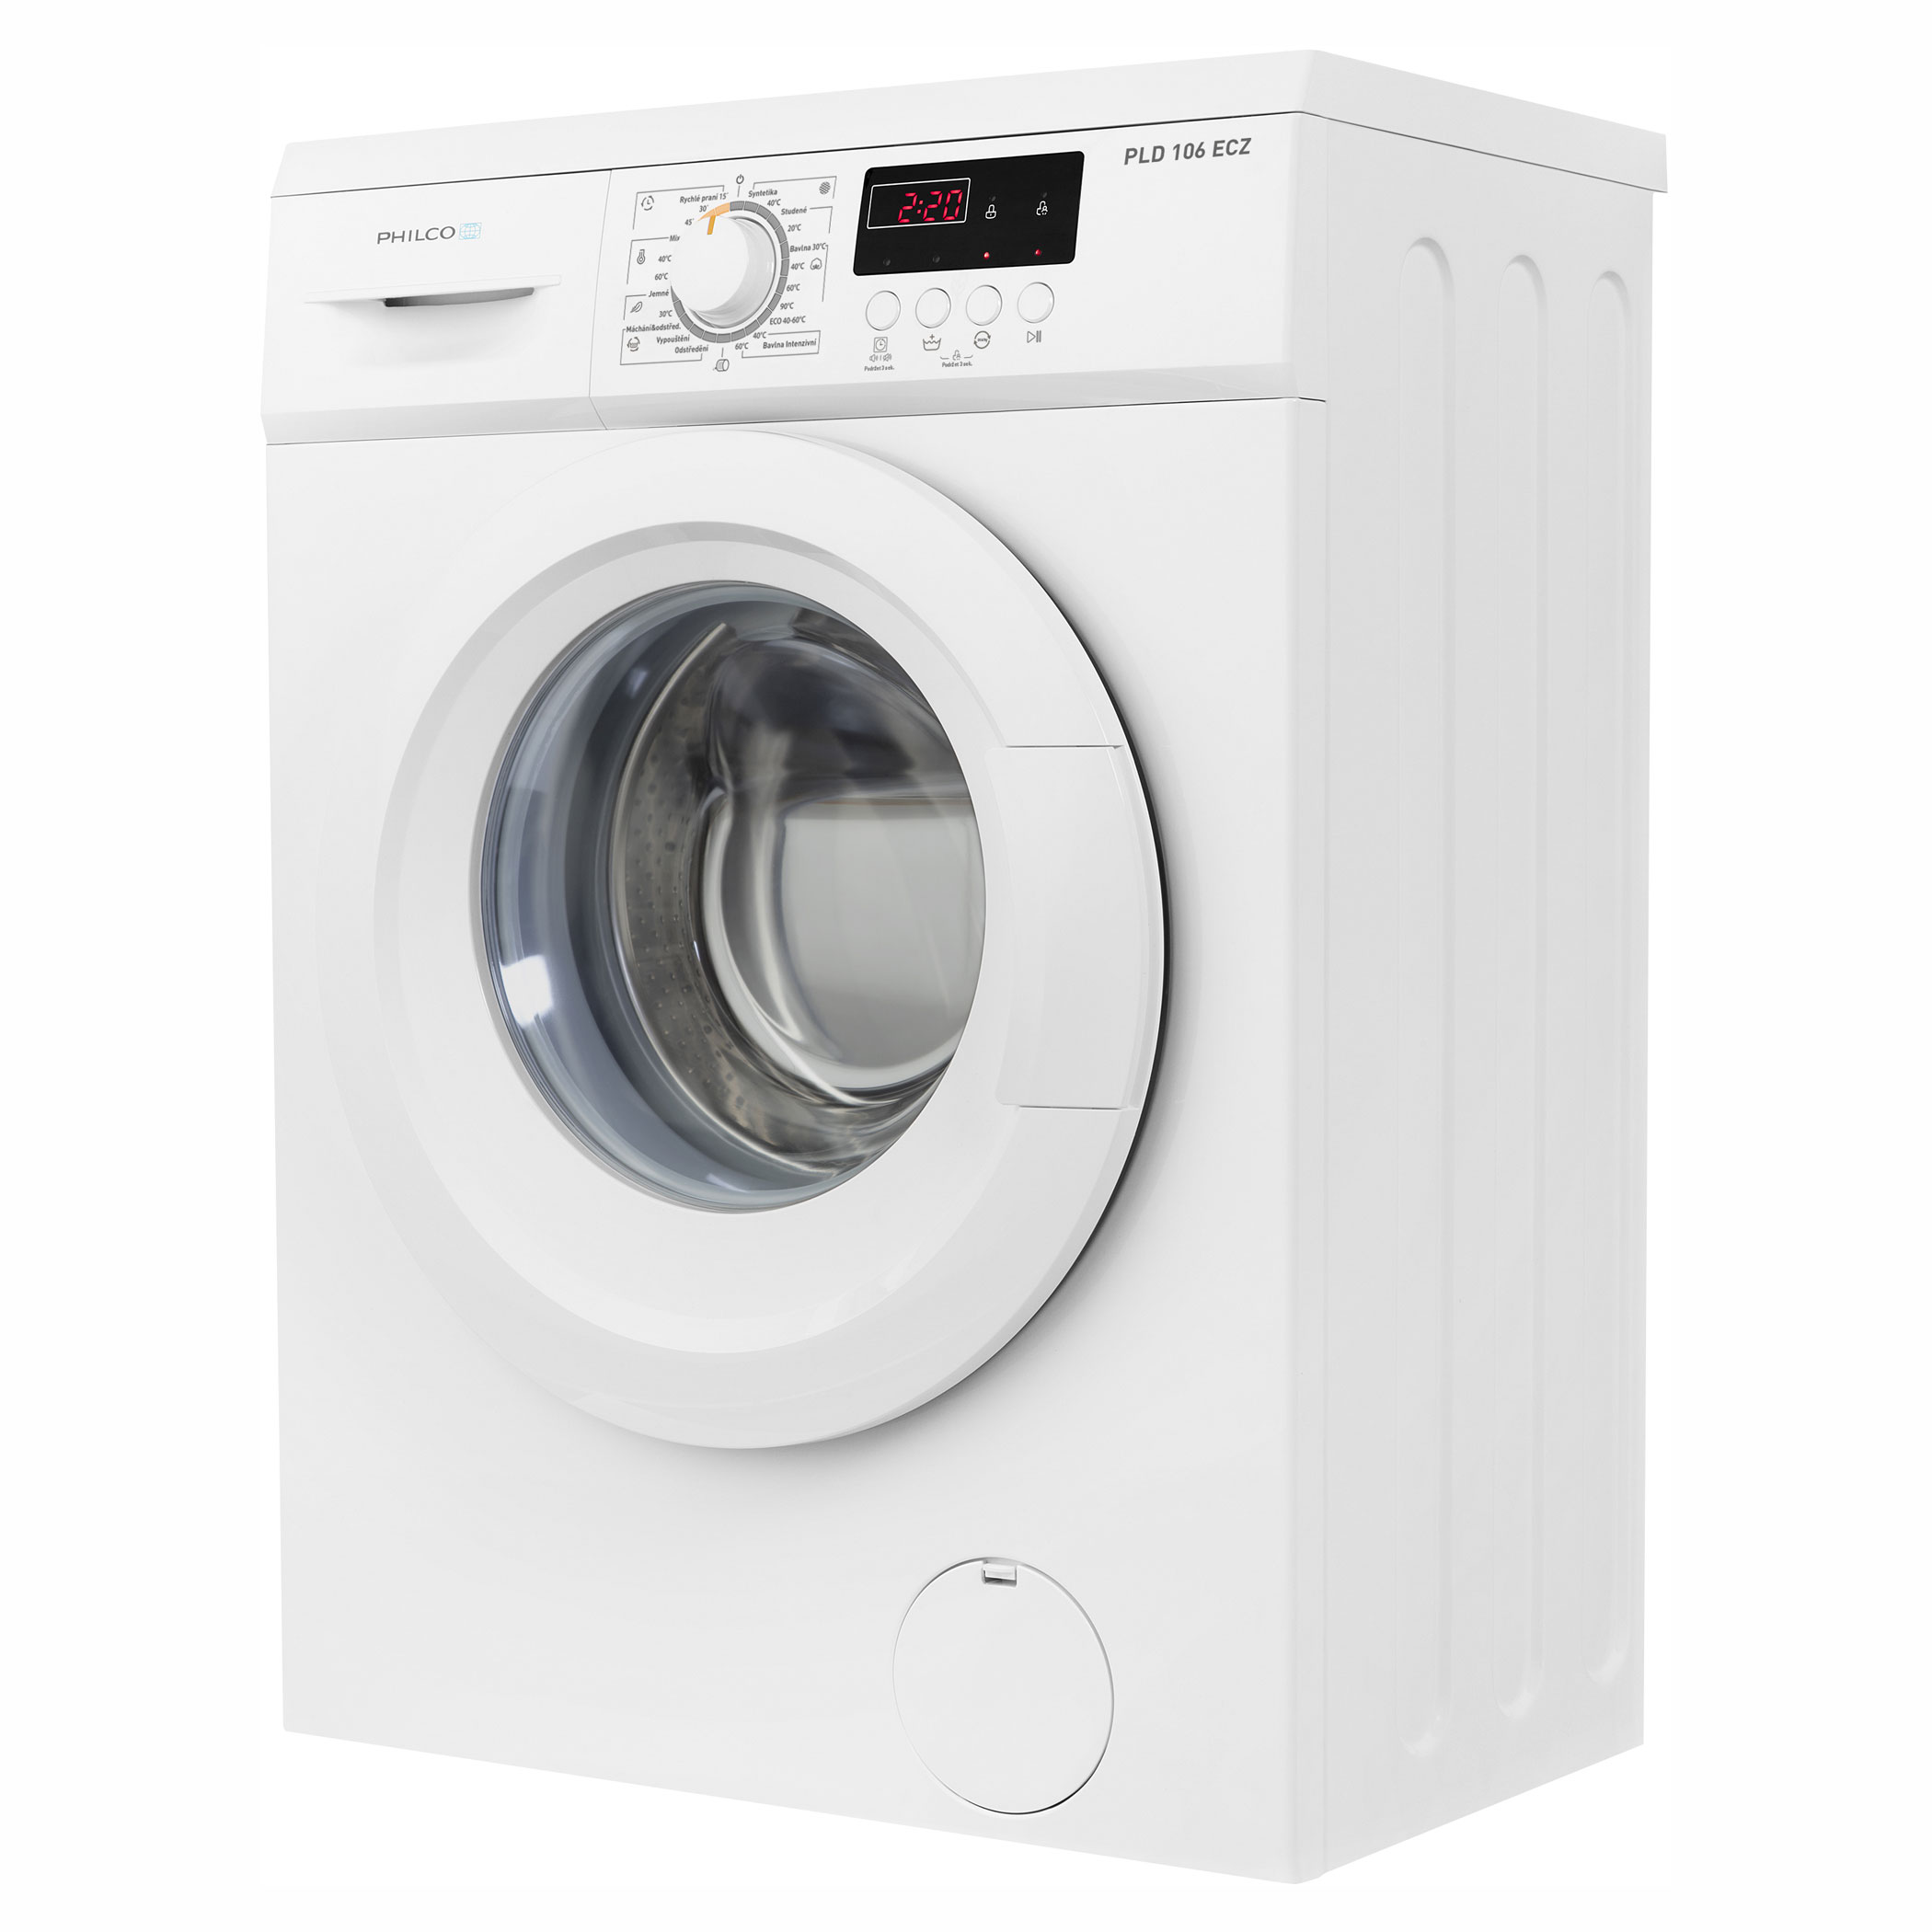
\includegraphics[
        width=3.20cm,
        height=3.35cm,
        keepaspectratio
    ]{figures/p01/pracka.jpg}
};

% Priemyselný robot
\node[inner sep=0pt] at (4.85,3.55) {
    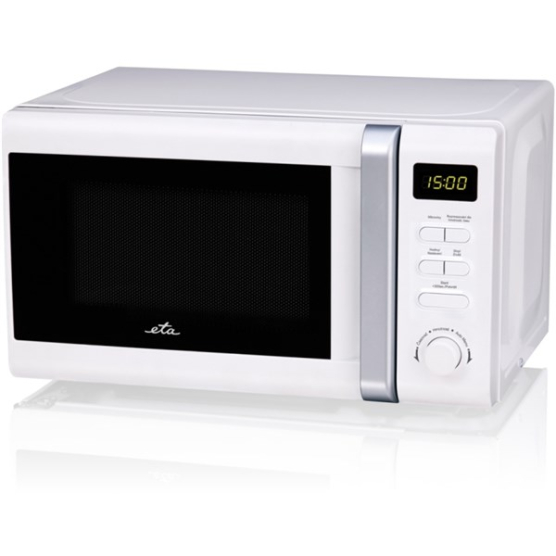
\includegraphics[
        width=3.90cm,
        height=3.25cm,
        keepaspectratio
    ]{figures/p01/mikrovlnka.jpg}
};

% Automobil
\node[inner sep=0pt] at (8.35,3.55) {
    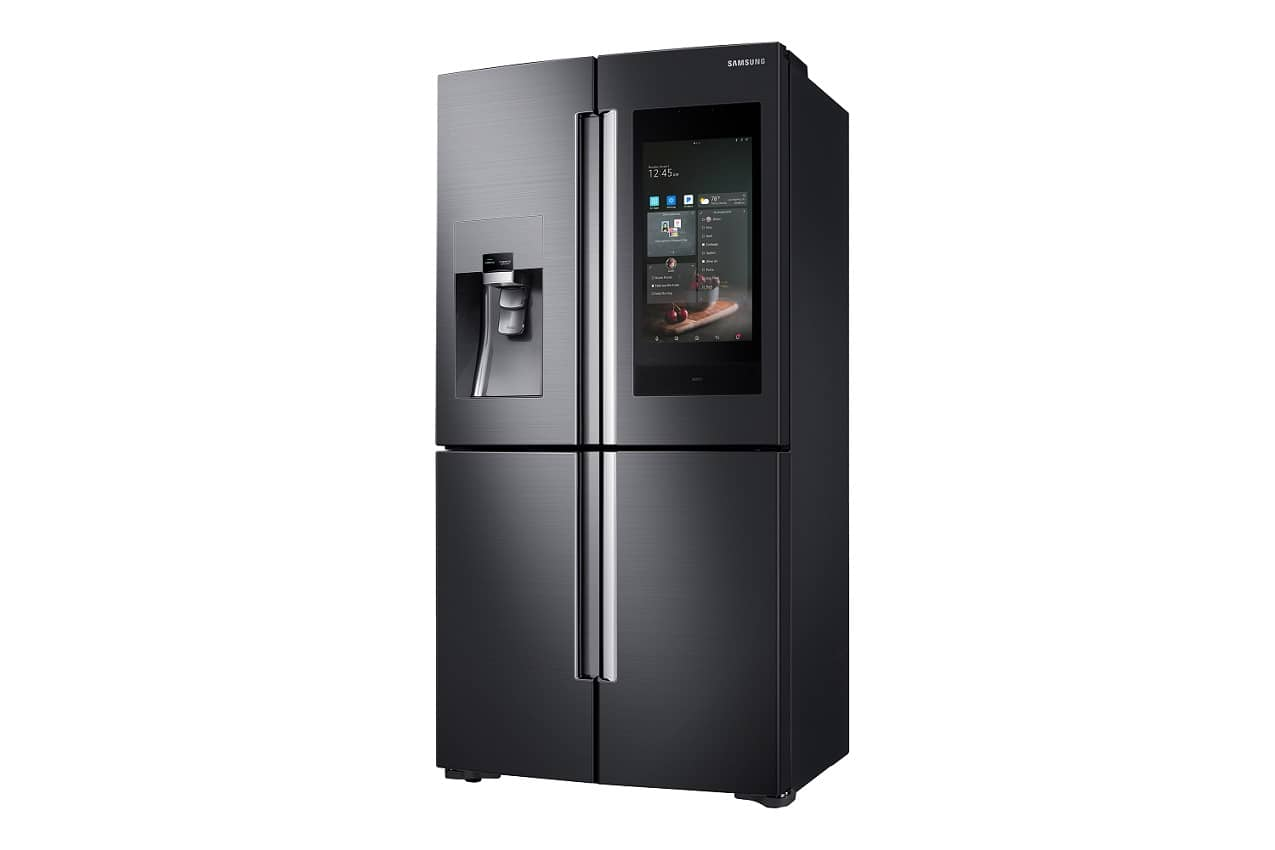
\includegraphics[
        width=3.10cm,
        height=3.20cm,
        keepaspectratio
    ]{figures/p01/chladnicka.jpg}
};

% Medicínske zariadenie
\node[inner sep=0pt] at (11.85,3.55) {
    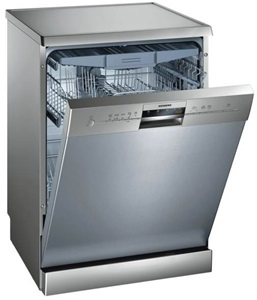
\includegraphics[
        width=3.75cm,
        height=3.25cm,
        keepaspectratio
    ]{figures/p01/umyvacka.jpg}
};

% ============================================================
% DOLNÝ RIADOK
% ============================================================

% Mobilné zariadenie
\node[inner sep=0pt] at (1.45,0.65) {
    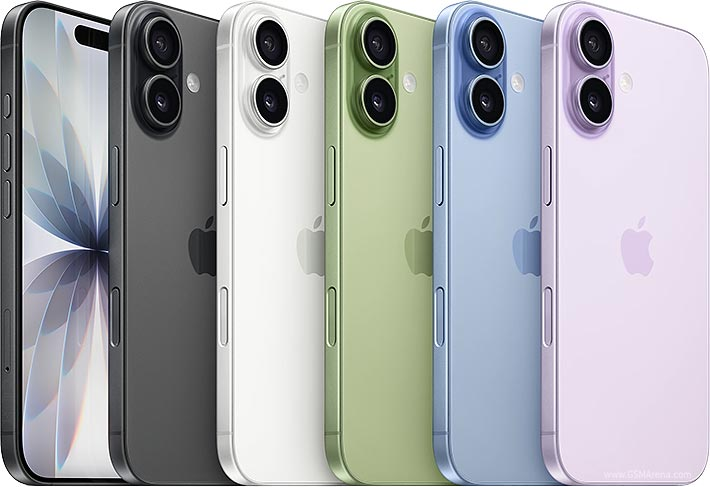
\includegraphics[
        width=2.55cm,
        height=3.35cm,
        keepaspectratio
    ]{figures/p01/iphone.jpg}
};

% Dron
\node[inner sep=0pt] at (4.85,0.65) {
    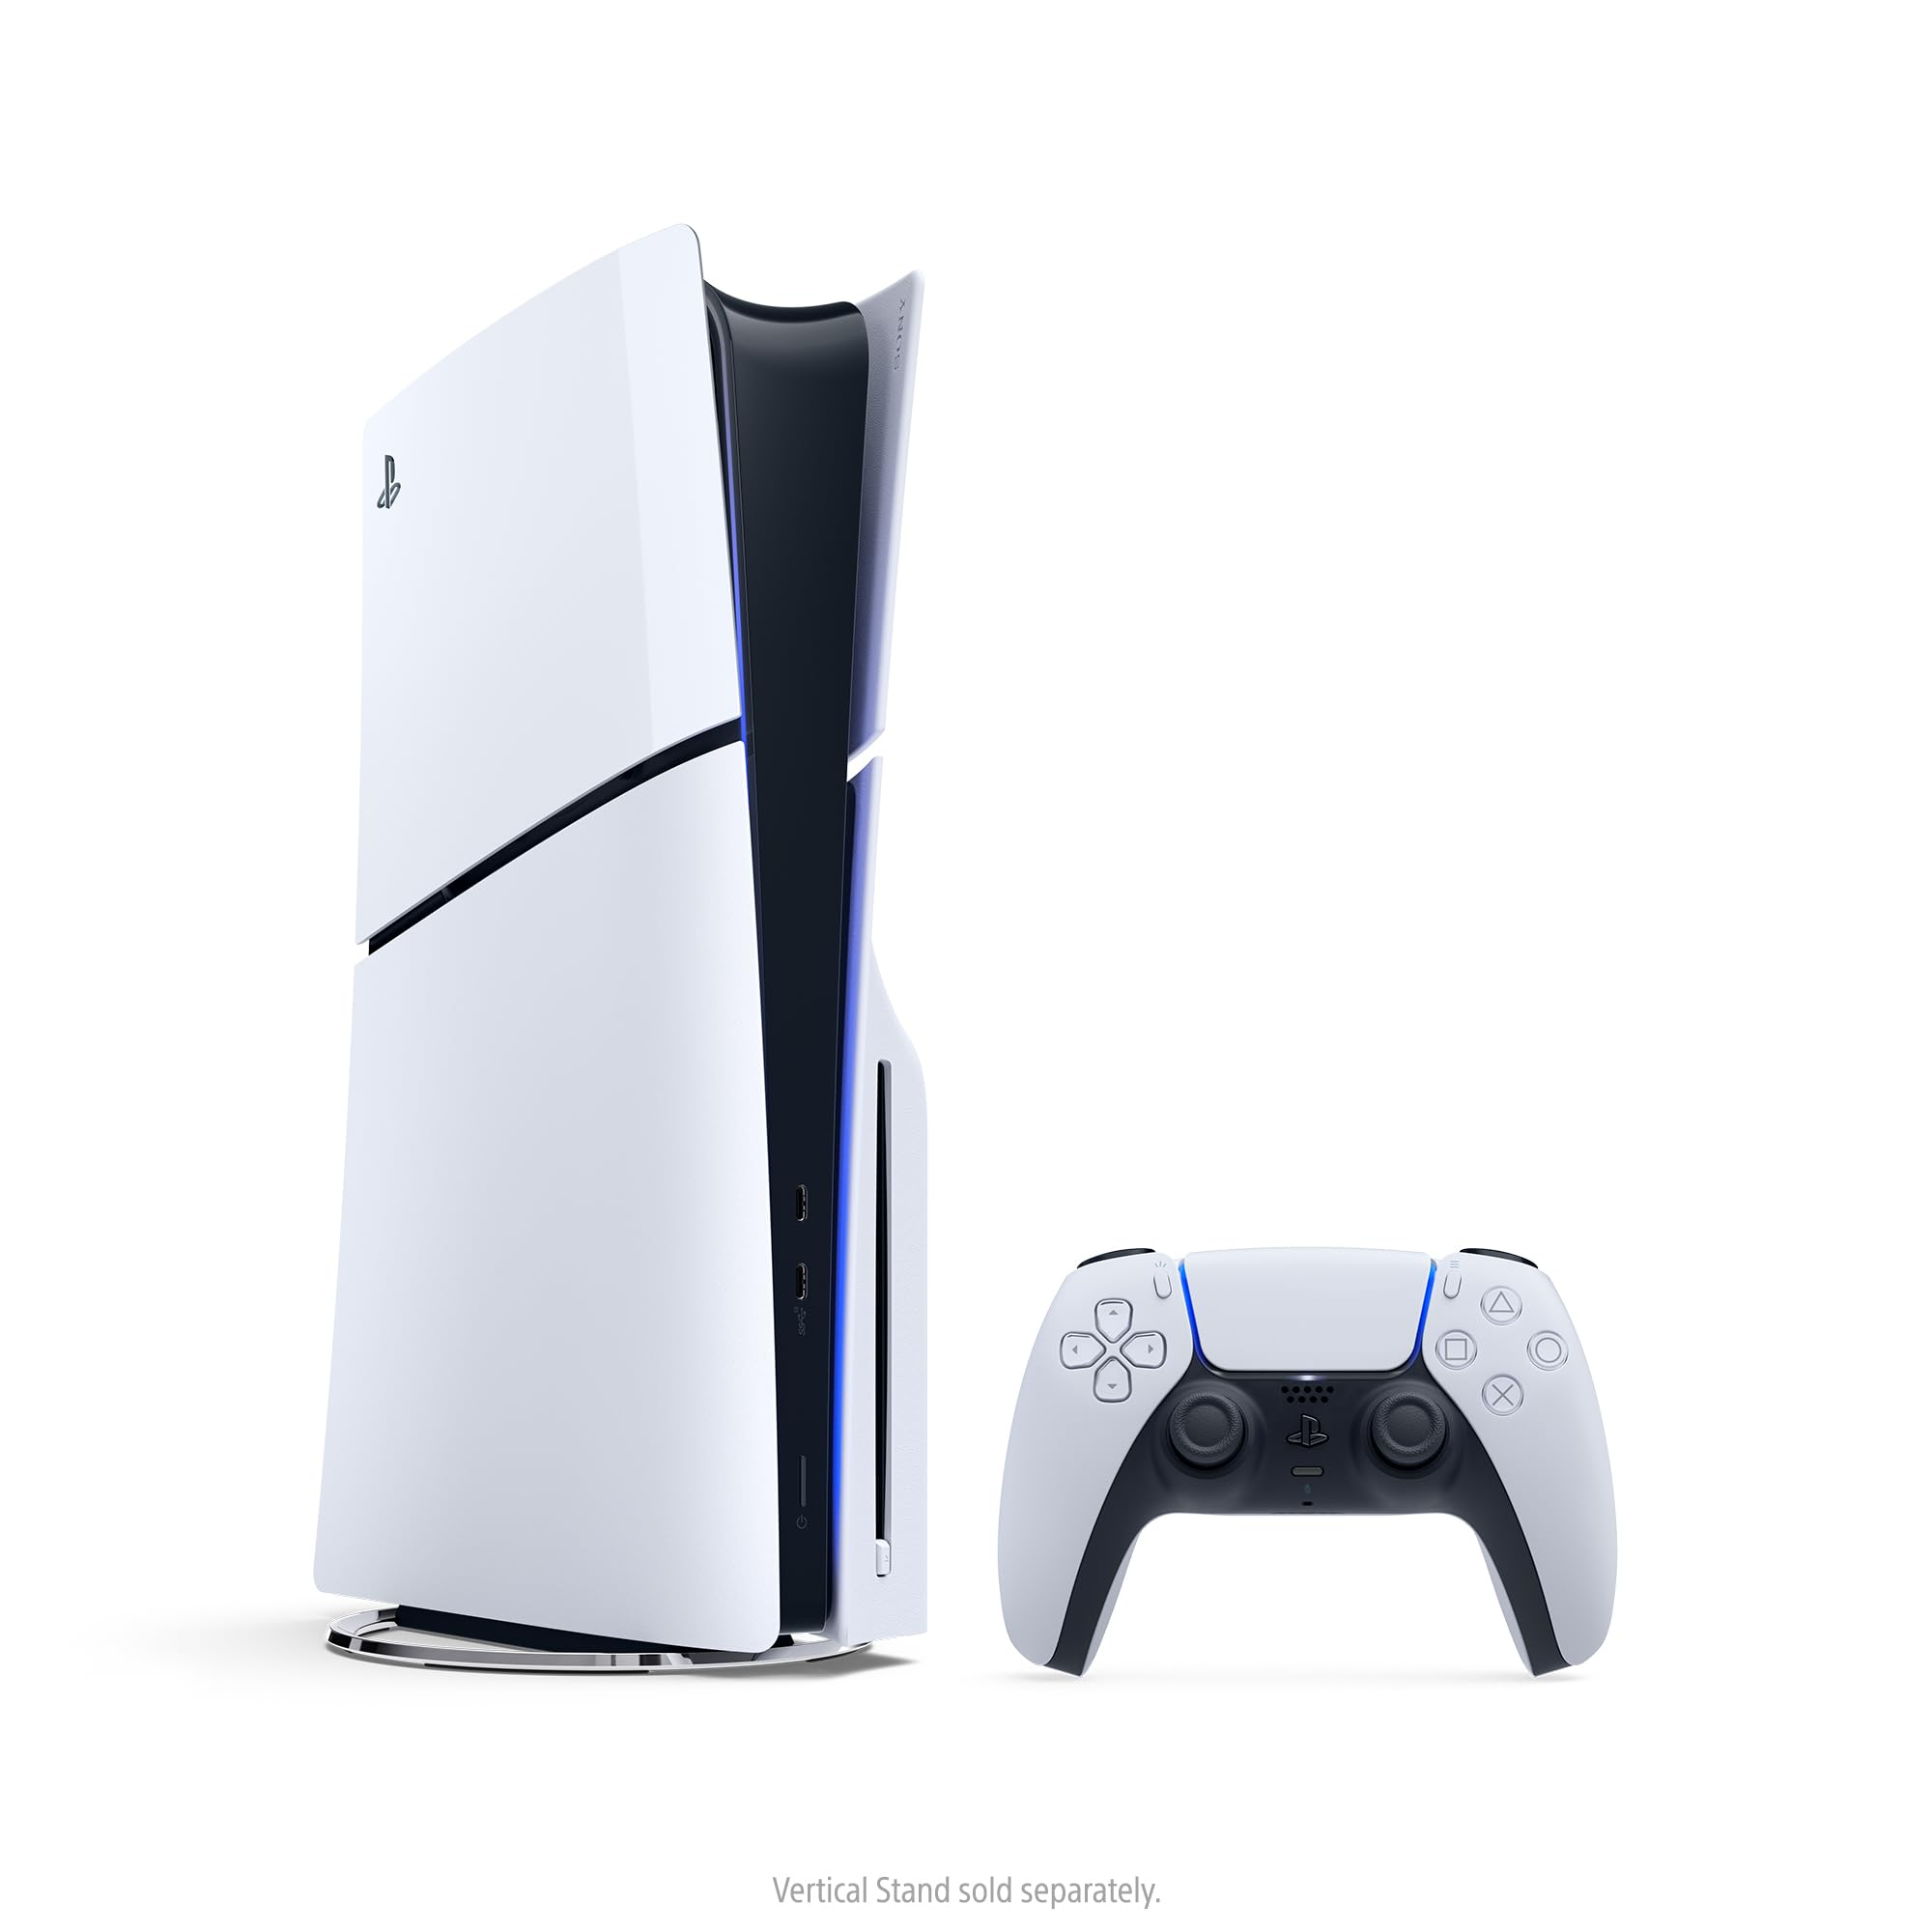
\includegraphics[
        width=3.85cm,
        height=3.15cm,
        keepaspectratio
    ]{figures/p01/ps5.jpg}
};

% Inteligentná domácnosť
\node[inner sep=0pt] at (8.35,0.65) {
    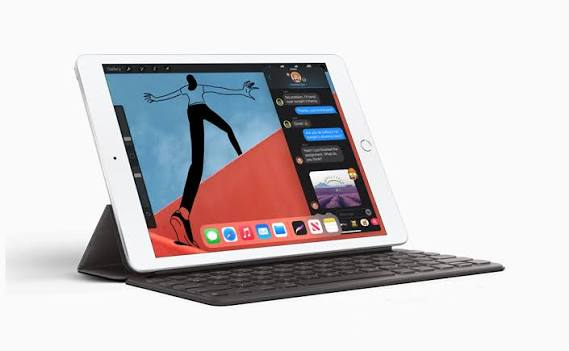
\includegraphics[
        width=4.15cm,
        height=3.15cm,
        keepaspectratio
    ]{figures/p01/ipad.jpeg}
};

% Lietadlo / letecké systémy
\node[inner sep=0pt] at (11.85,0.65) {
    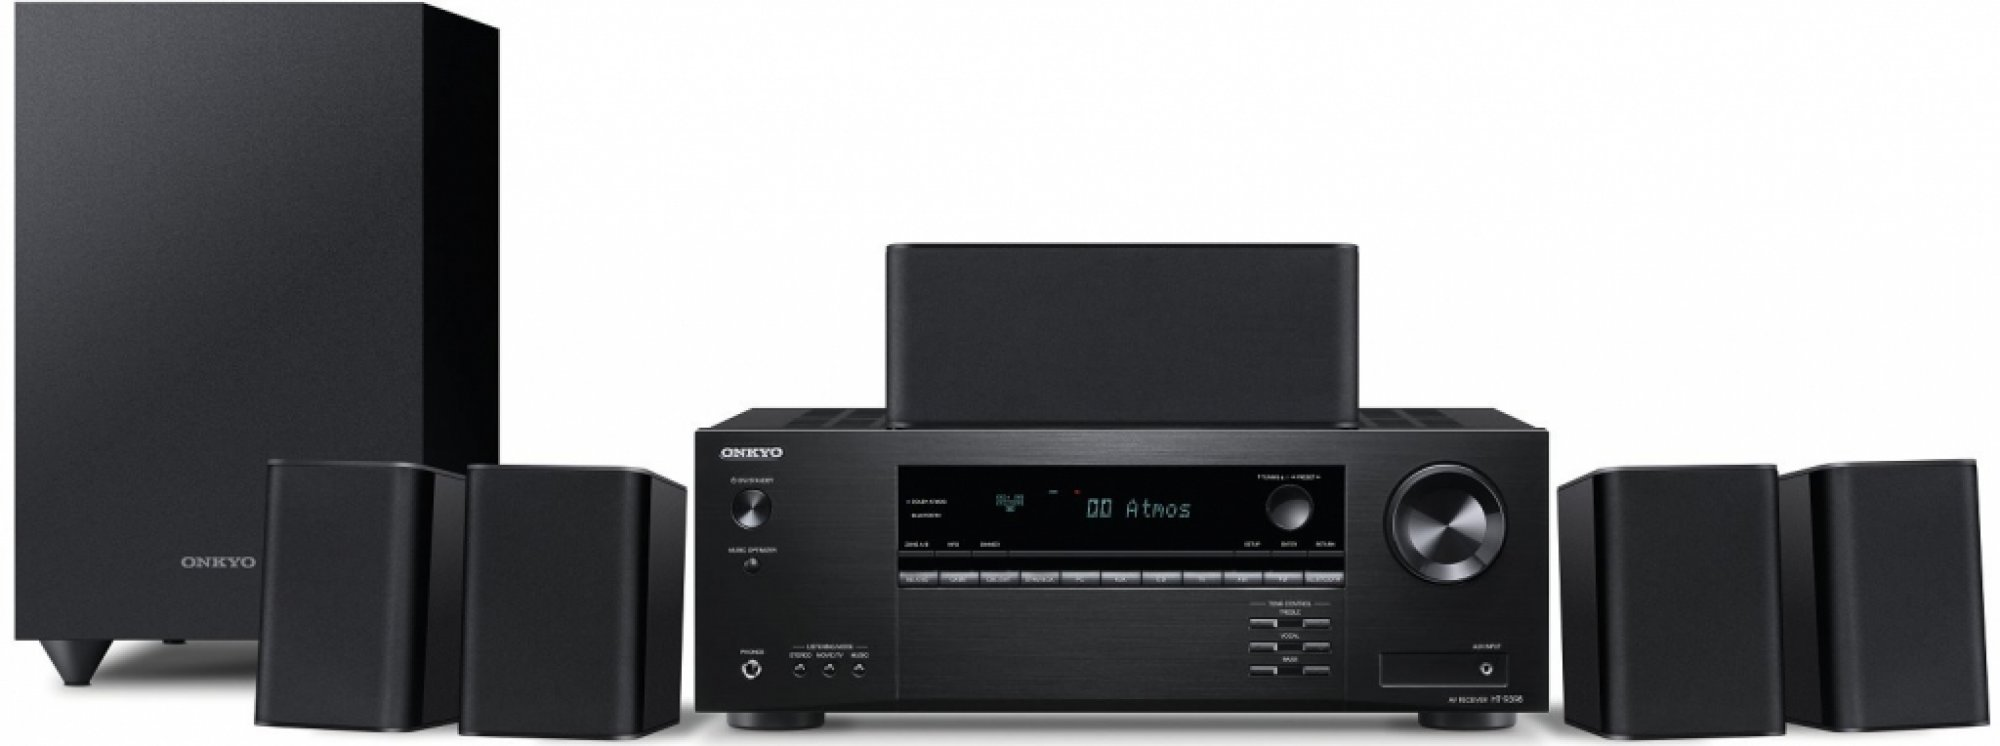
\includegraphics[
        width=3.95cm,
        height=3.15cm,
        keepaspectratio
    ]{figures/p01/domaceKino.jpg}
};

\end{tikzpicture}
\end{frame}

\begin{frame}{Využitie mikrokontrolérov v praxi}

\centering
\vspace{-0.10cm}

\begin{tikzpicture}[x=1cm,y=1cm]

% Pevná plocha obrázkovej koláže
% Zabraňuje posúvaniu alebo presahovaniu obrázkov.
\path[use as bounding box]
    (-0.2,-0.80) rectangle (13.6,4.85);

% ============================================================
% HORNÝ RIADOK
% ============================================================

% Práčka / domáci spotrebič
\node[inner sep=0pt] at (1.45,3.55) {
    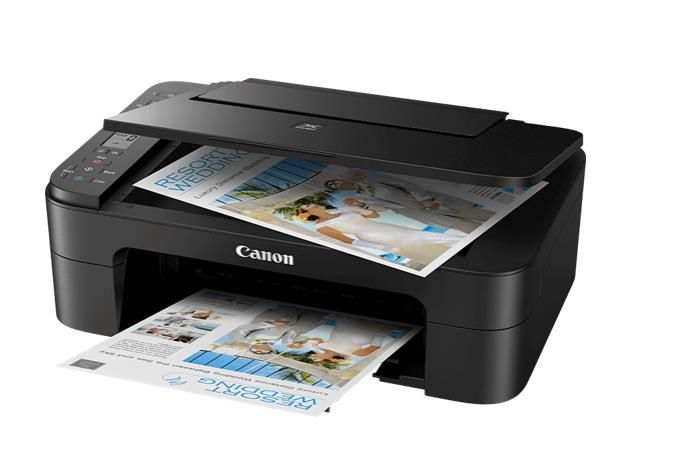
\includegraphics[
        width=3.20cm,
        height=4.35cm,
        keepaspectratio
    ]{figures/p01/tlaciaren.jpg}
};

% Priemyselný robot
\node[inner sep=0pt] at (4.85,3.55) {
    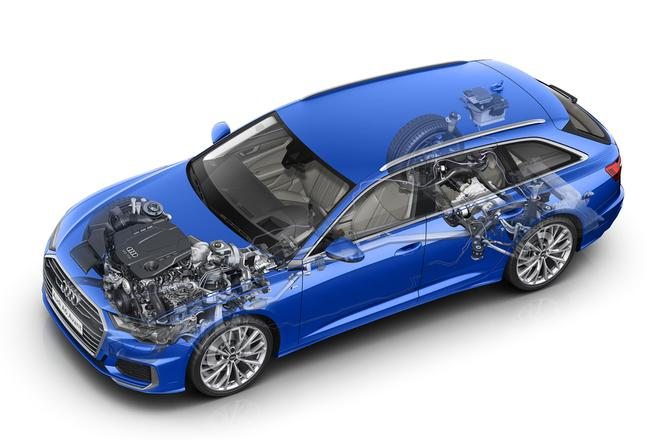
\includegraphics[
        width=3.90cm,
        height=3.25cm,
        keepaspectratio
    ]{figures/p01/auto.jpg}
};

% Automobil
\node[inner sep=0pt] at (8.35,3.55) {
    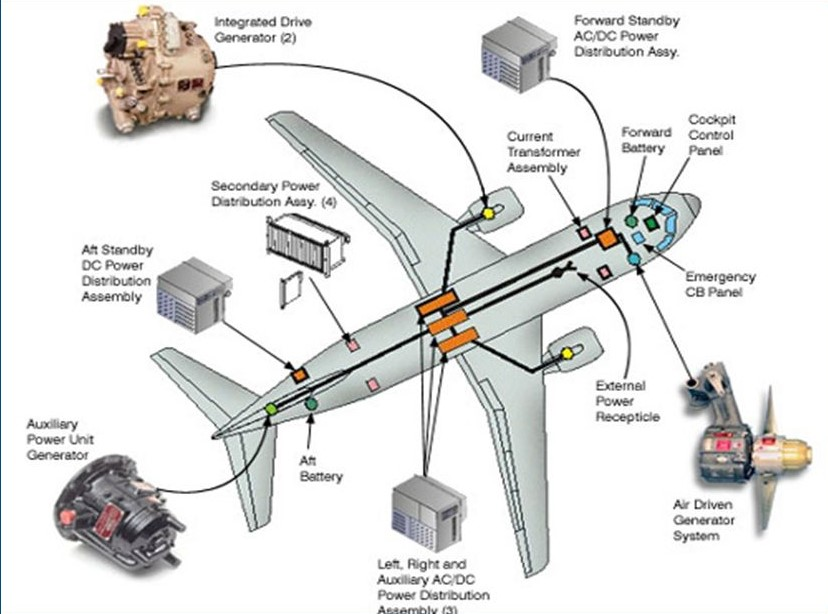
\includegraphics[
        width=3.10cm,
        height=3.20cm,
        keepaspectratio
    ]{figures/p01/lietadlo.png}
};

% Military
\node[inner sep=0pt] at (11.85,3.55) {
    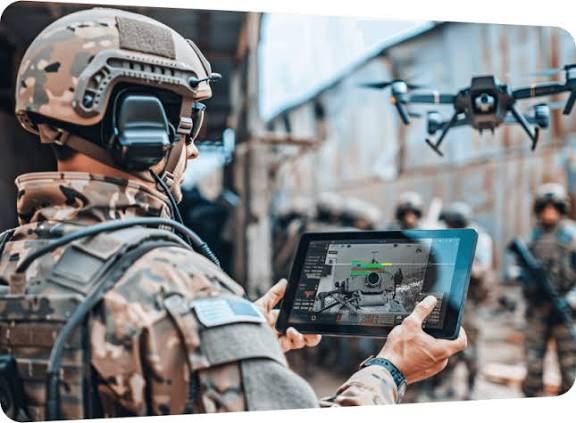
\includegraphics[
        width=3.10cm,
        height=3.20cm,
        keepaspectratio
    ]{figures/p01/military.jpeg}
};


% ============================================================
% DOLNÝ RIADOK
% ============================================================

% Mobilné zariadenie
\node[inner sep=0pt] at (1.45,0.65) {
    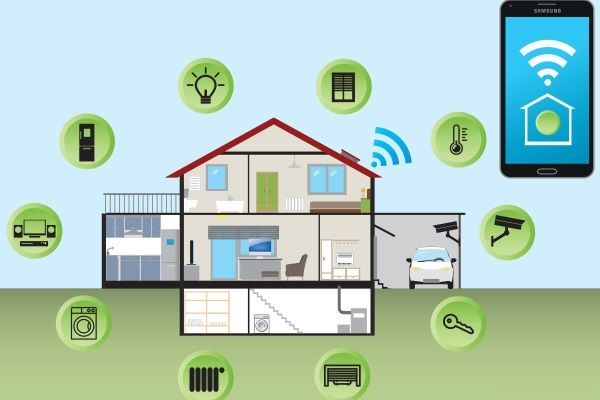
\includegraphics[
        width=2.55cm,
        height=3.35cm,
        keepaspectratio
    ]{figures/p01/dom.jpg}
};

% Dron
\node[inner sep=0pt] at (4.85,0.65) {
    \includegraphics[
        width=3.85cm,
        height=3.15cm,
        keepaspectratio
    ]{figures/p01/davinci.jpg}
};

% Inteligentná domácnosť
\node[inner sep=0pt] at (8.35,0.65) {
    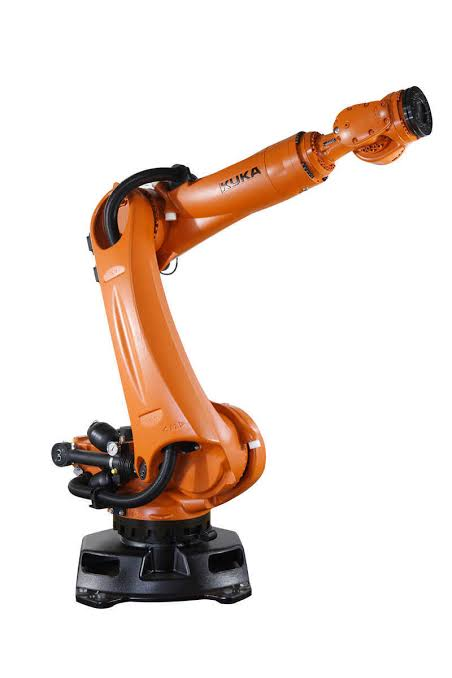
\includegraphics[
        width=4.15cm,
        height=3.15cm,
        keepaspectratio
    ]{figures/p01/kuka.jpeg}
};

% Lietadlo / letecké systémy
\node[inner sep=0pt] at (11.85,0.65) {
    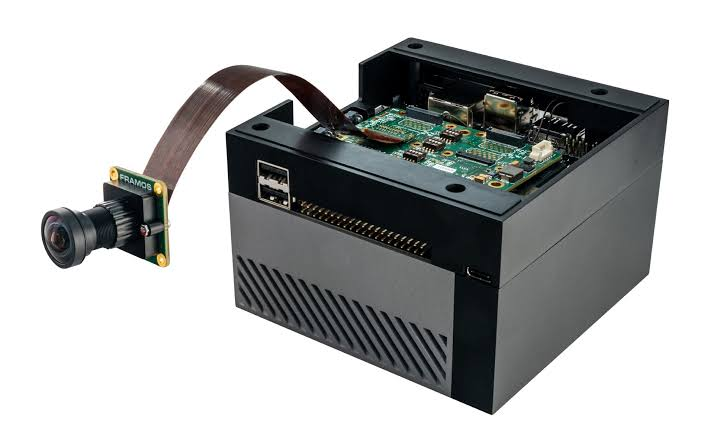
\includegraphics[
        width=3.95cm,
        height=3.15cm,
        keepaspectratio
    ]{figures/p01/camera.jpeg}
};

\end{tikzpicture}
\end{frame}
\SectionFrame{1. Historická línia}{Od pevne zapojenej logiky k programovateľnému riadiacemu systému}

\begin{frame}{Pevne zapojená logika: riadiaci algoritmus ako zapojenie}

\begin{columns}[T,onlytextwidth]

\column{0.52\textwidth}

\BlueBox{\faIcon[regular]{lightbulb}\hspace{0.5em}Podstata}{
Pri pevne zapojenej logike je postup riadenia daný fyzickým prepojením
kontaktov, relé, tlačidiel, časových relé a výkonových prvkov.
}

\vspace{0.15cm}

\begin{itemize}
    \item riadiaca logika je zapísaná v elektrickej schéme,
    \item zmena algoritmu znamená zmenu zapojenia,
    \item vhodné pre jednoduché a stabilné úlohy,
    \item pri zložitejšom riadení rastie počet vodičov, relé a porúch,
    \item programovateľné riadiace systémy vznikli ako odpoveď na túto zložitosť.
\end{itemize}

\vspace{0.15cm}

\BlueBox{\faIcon{arrow-right}\hspace{0.5em}Prechod}{
Od otázky „ako to zapojiť?“ sa vývoj posunul k otázke
„ako to naprogramovať?“
}

\column{0.43\textwidth}

\centering

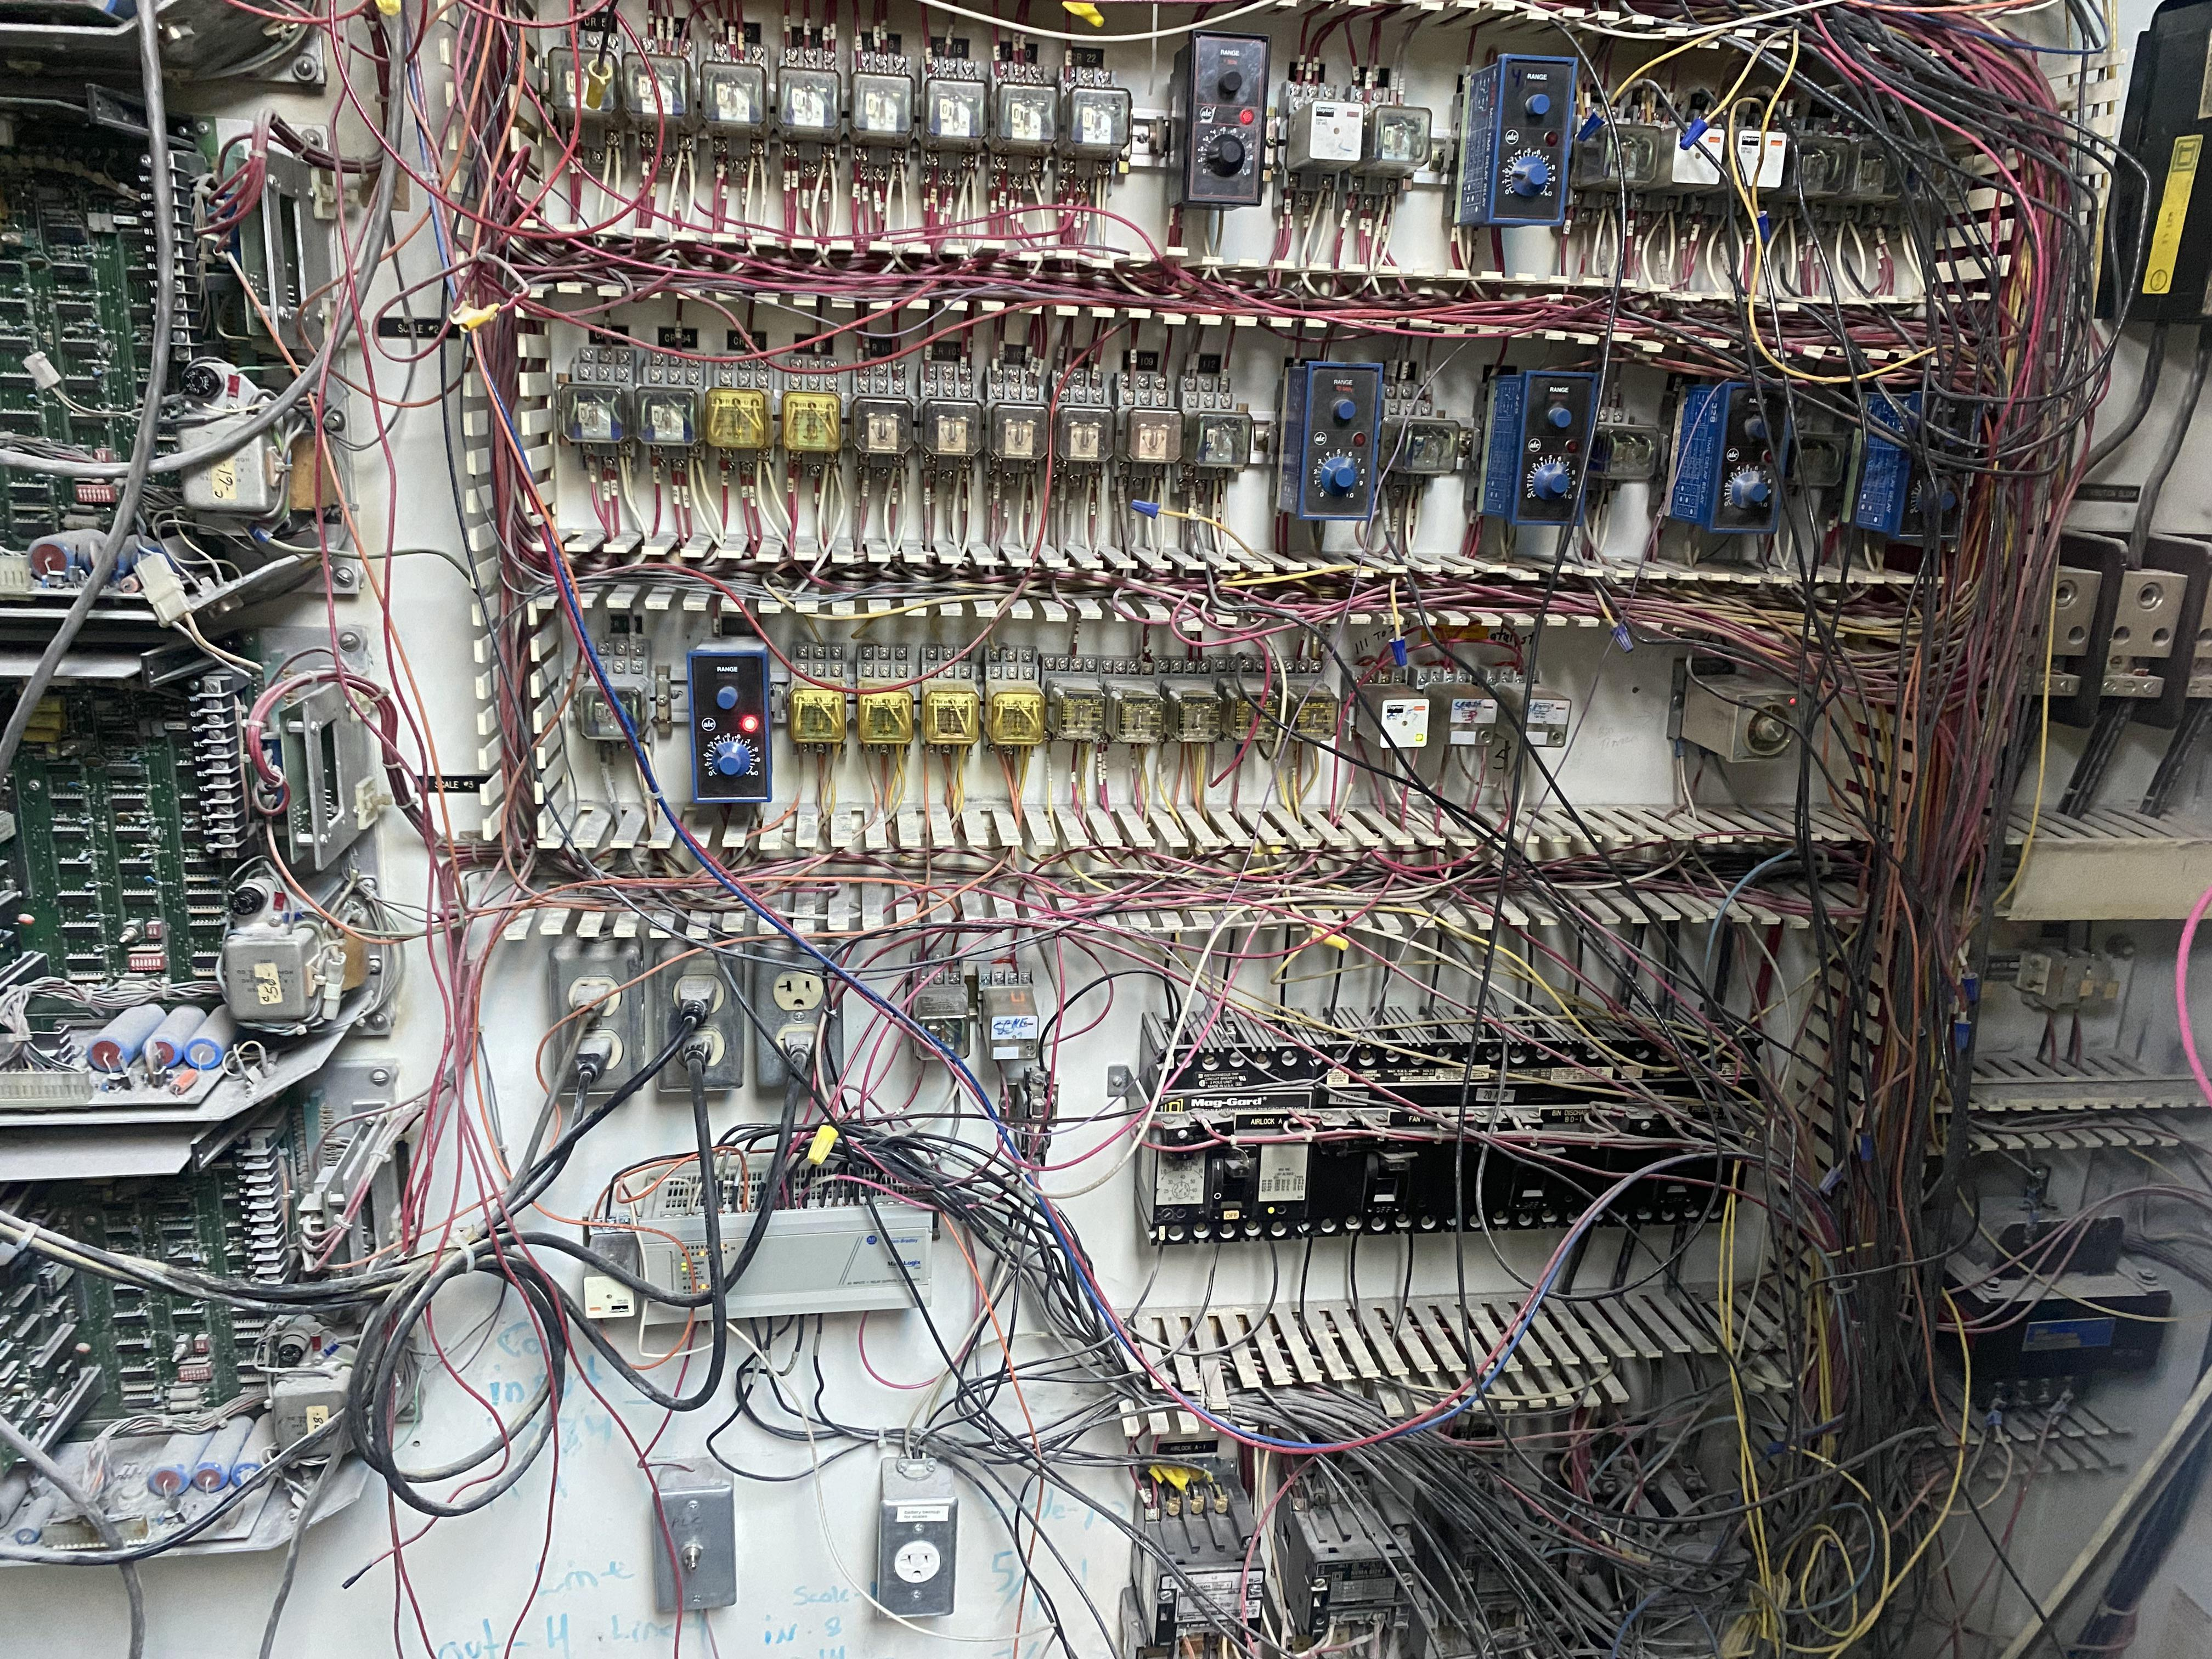
\includegraphics[
    width=\linewidth,
    height=0.39\textheight,
    keepaspectratio
]{figures/p01/rele.jpeg}

\vspace{0.25cm}

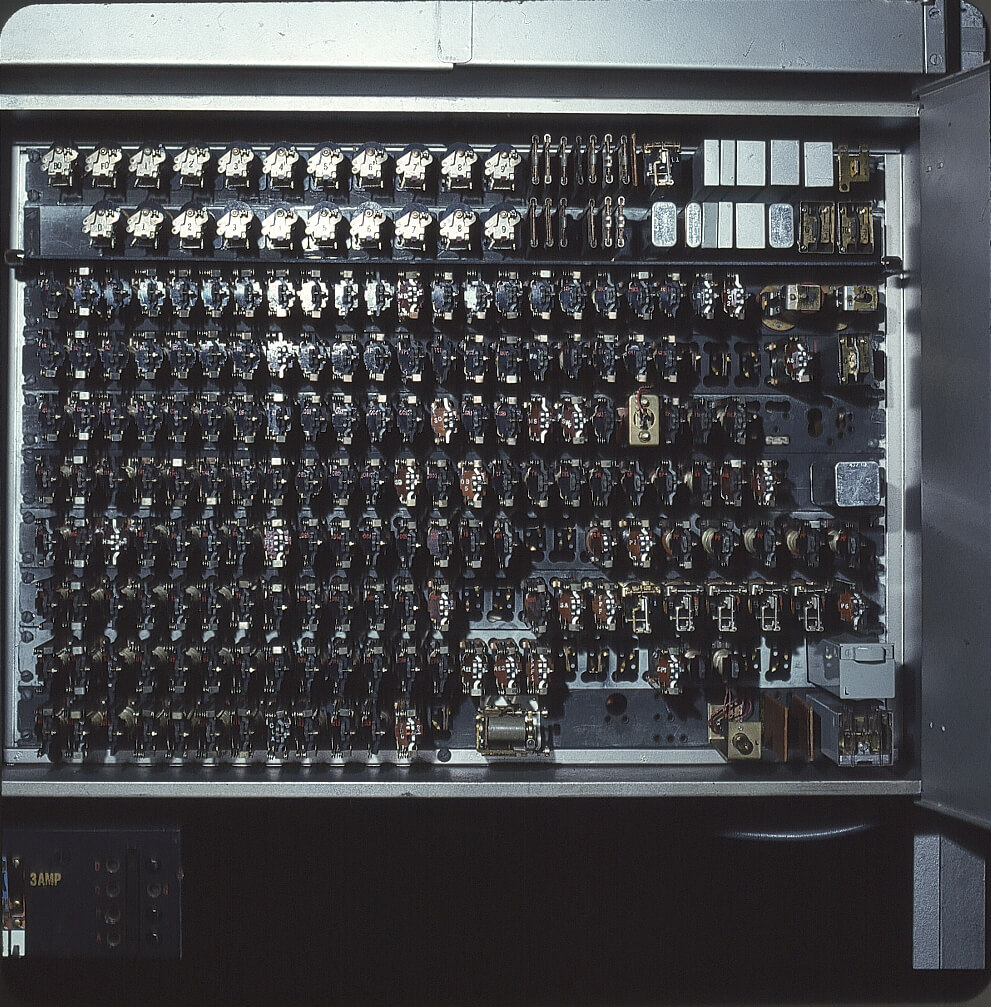
\includegraphics[
    width=\linewidth,
    height=0.39\textheight,
    keepaspectratio
]{figures/p01/rele2.jpg}

\vspace{0.12cm}

\end{columns}

\end{frame}

\begin{frame}{Colossus: špecializovaný elektronický výpočet}
\begin{columns}[T,onlytextwidth]
\column{0.47\textwidth}
\begin{itemize}
  \item 1943/1944: elektronický stroj pre kryptografickú analýzu.
  \item Ukázal, že rozsiahla logická úloha sa dá riešiť rýchlejšie elektronicky než mechanicky.
  \item Nebol to mikrokontrolér, ale ukazuje prechod od mechaniky k elektronickej logike.
\end{itemize}
\BlueBox{
    \faIcon{microchip}\hspace{0.5em}Základná myšlienka
}{
    Rýchlosť logiky začala byť určovaná elektronikou, nie pohybom mechanických kontaktov.
}
% ============================================================
% PRAVÝ STĹPEC – ŠTYRI OBRÁZKY
% ============================================================
\column{0.43\textwidth}

\centering
\vspace{0.10cm}

% Horný riadok
\begin{minipage}[t]{0.48\linewidth}
    \centering
    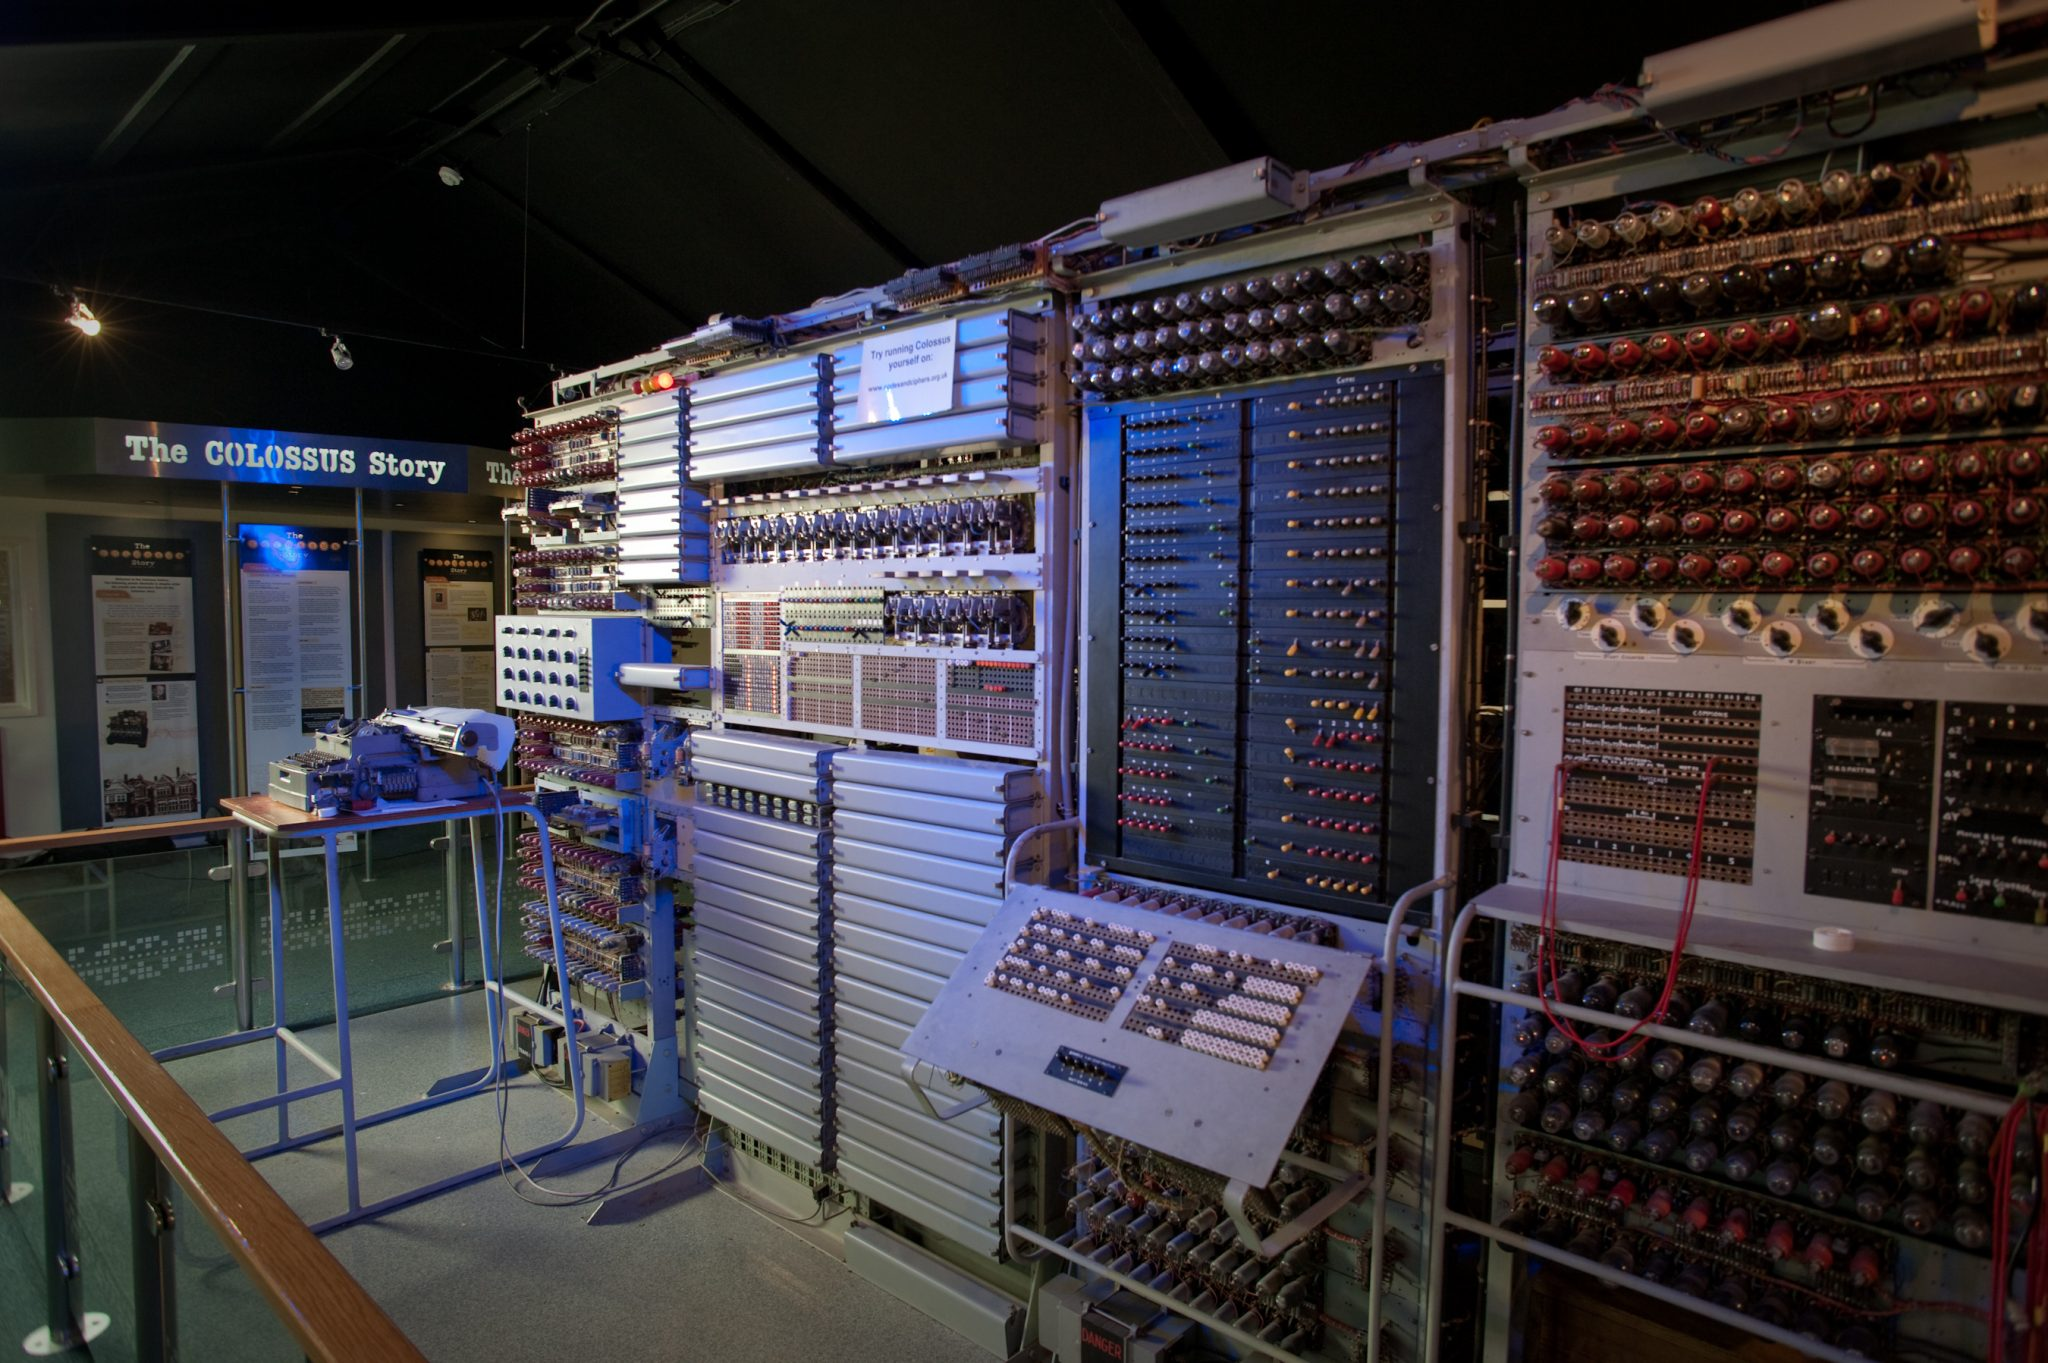
\includegraphics[
        width=\linewidth,
        height=0.35\textheight,
        keepaspectratio
    ]{figures/p01/colossus.jpg}
\end{minipage}
\hfill
\begin{minipage}[t]{0.48\linewidth}
    \centering
    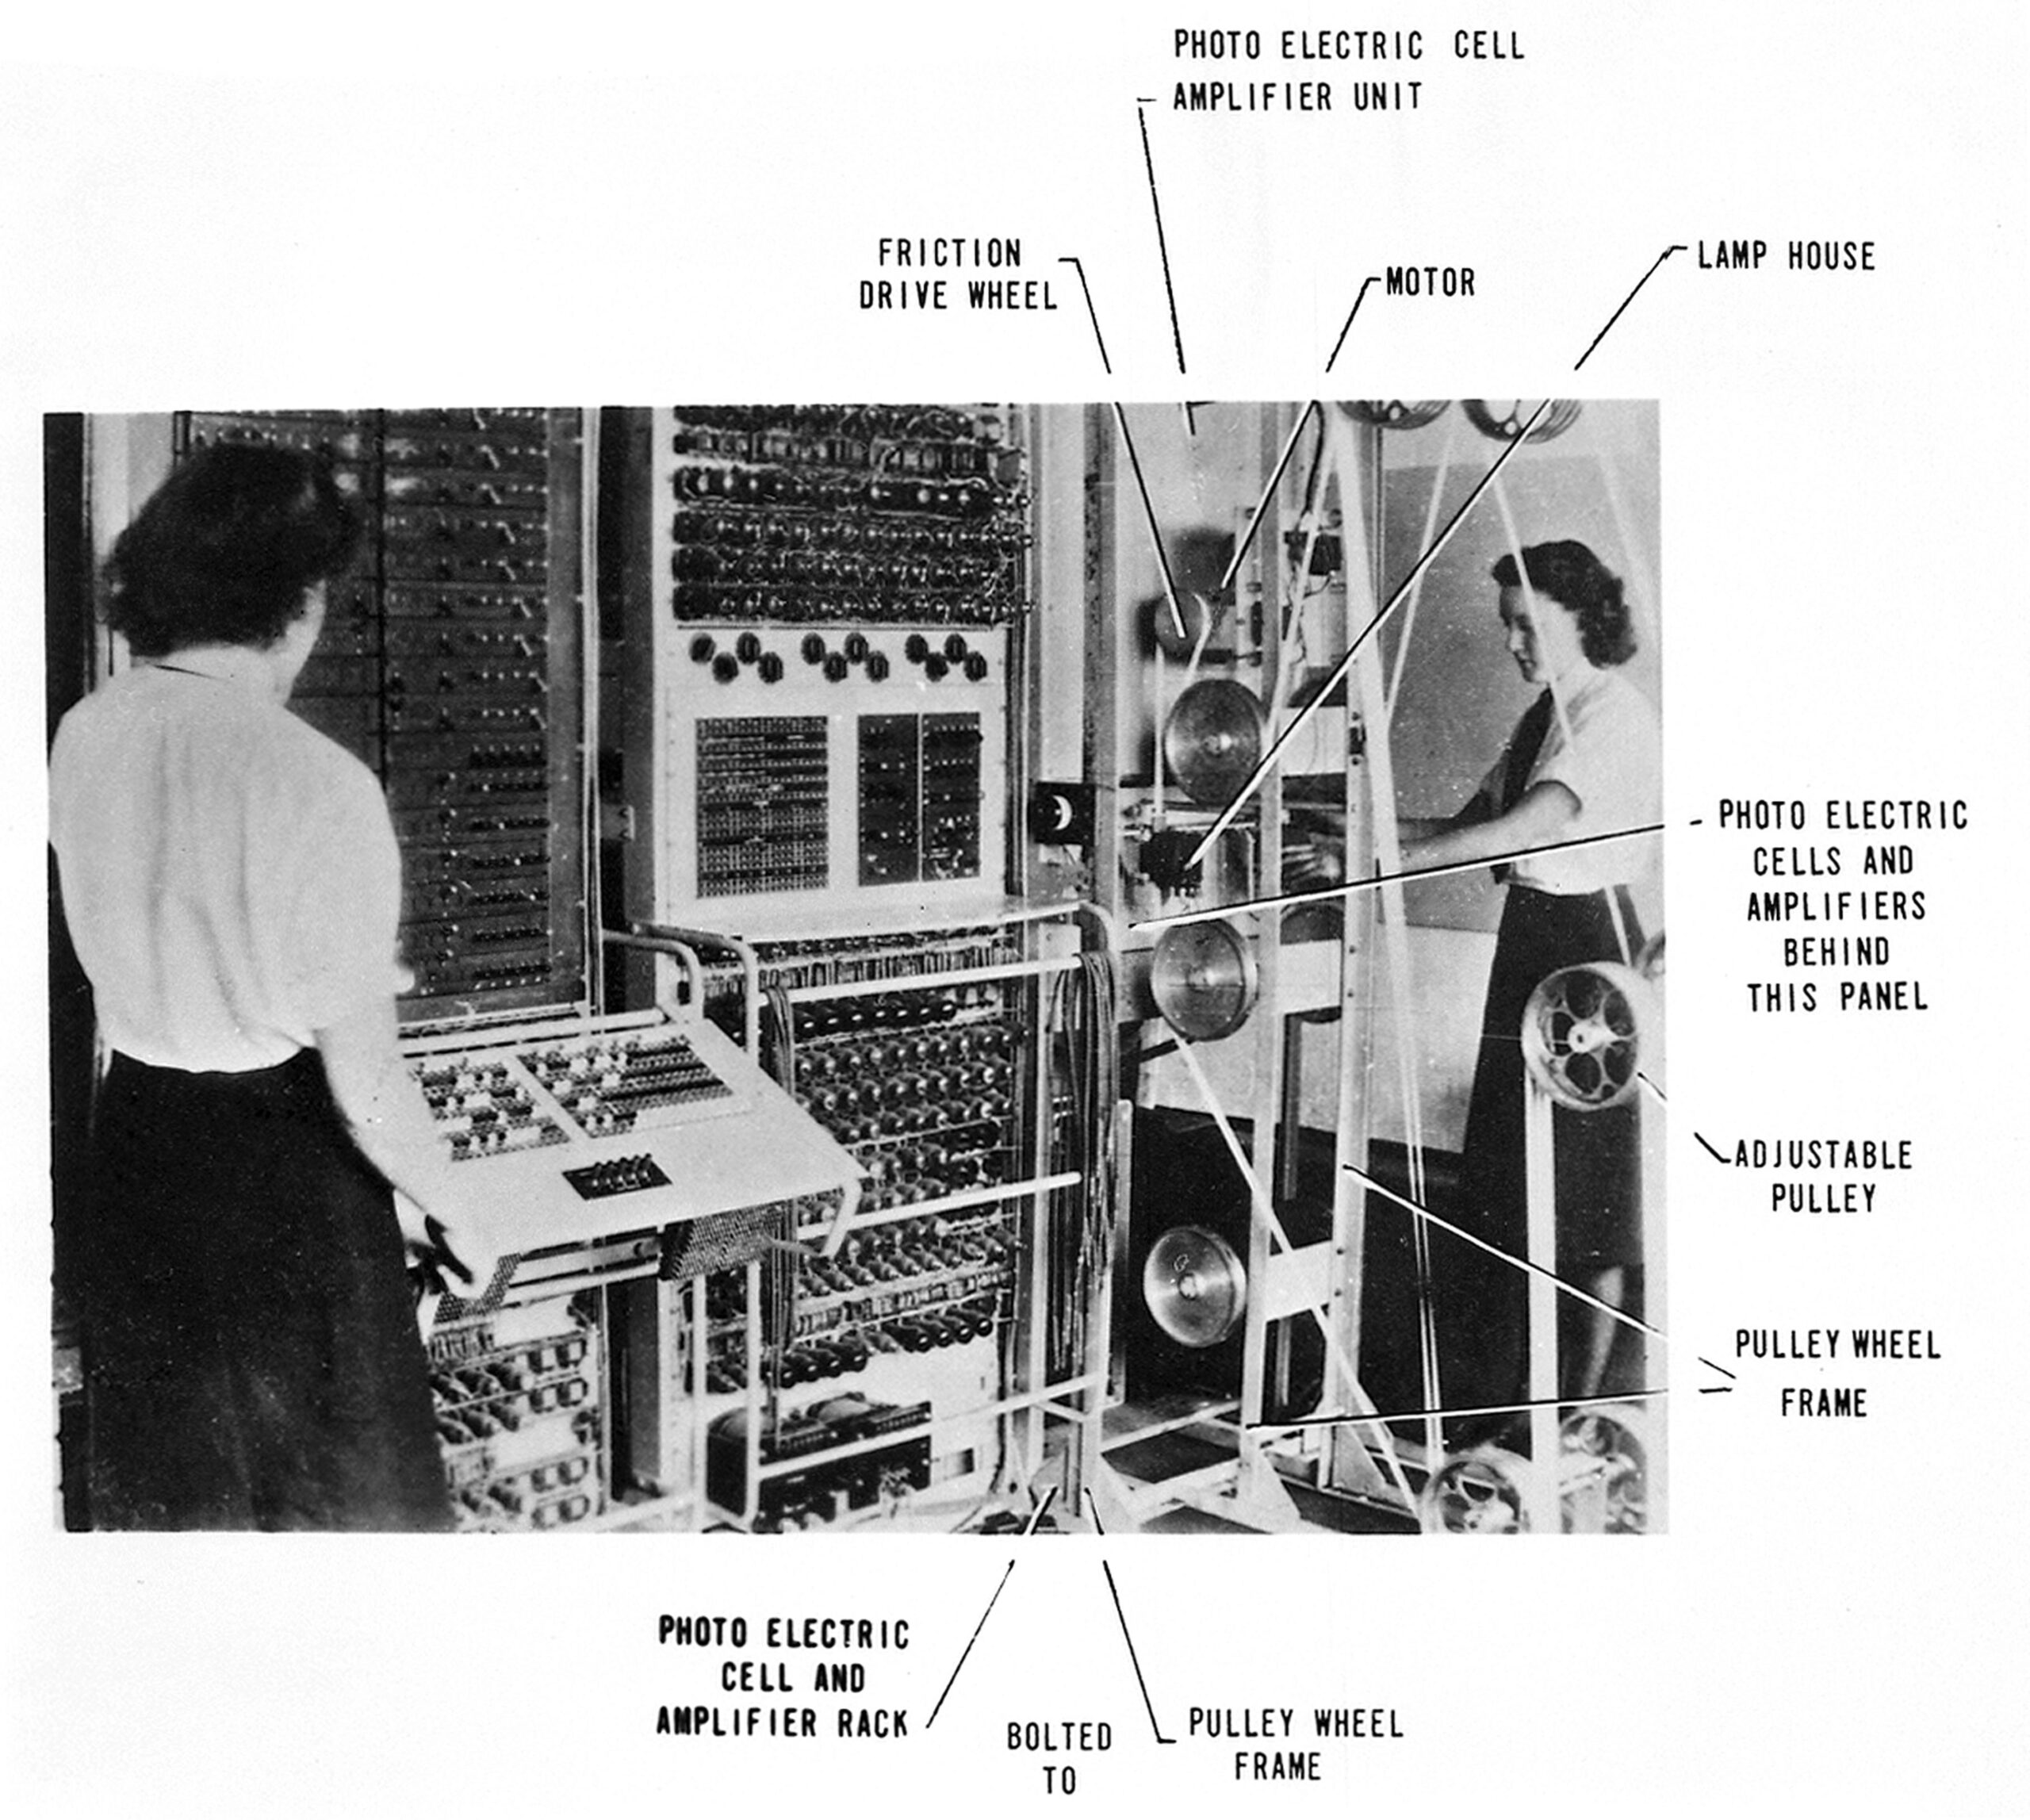
\includegraphics[
        width=\linewidth,
        height=0.35\textheight,
        keepaspectratio
    ]{figures/p01/colossus2.jpg}
\end{minipage}

\vspace{0.18cm}

% Dolný riadok
\begin{minipage}[t]{0.48\linewidth}
    \centering
    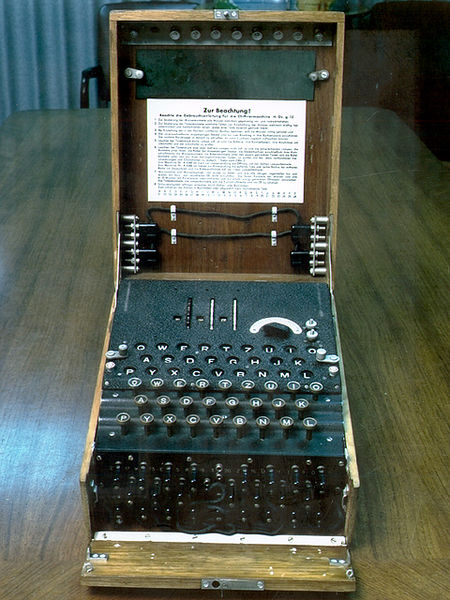
\includegraphics[
        width=\linewidth,
        height=0.35\textheight,
        keepaspectratio
    ]{figures/p01/enigma.jpg}
\end{minipage}
\hfill
\begin{minipage}[t]{0.48\linewidth}
    \centering
    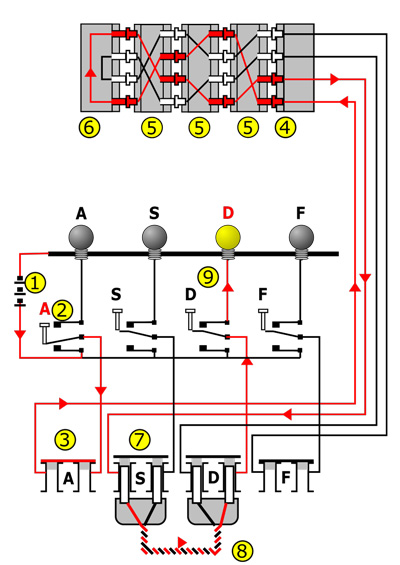
\includegraphics[
        width=\linewidth,
        height=0.35\textheight,
        keepaspectratio
    ]{figures/p01/enigma2.jpg}
\end{minipage}

\end{columns}
\end{frame}

\begin{frame}{ENIAC: elektromechanický počítač}
\begin{columns}[T,onlytextwidth]
\column{0.56\textwidth}
\begin{itemize}
  \item 1946: elektronický počítač založený na elektrónkach.
  \item Veľký výkon na svoju dobu, ale extrémne rozmery, spotreba a zložité programovanie.
  \item Programovanie často znamenalo prepájanie káblov a nastavovanie prepínačov.
  \item V r. 1948 upravený na čítanie z ROM: spomalenie výkonu 6-násobne, zmena dĺžky programovania z niekoľkých dní na hodiny
  \item Obsahoval: 21 501 elektróniek, 7200 kryštálových diód, 1500 relé, 70 000 rezistorov, 
     5 mil. ručne spájkovaných spojov, váha 30 t, rozmer 63 m2
\end{itemize}
\column{0.38\textwidth}
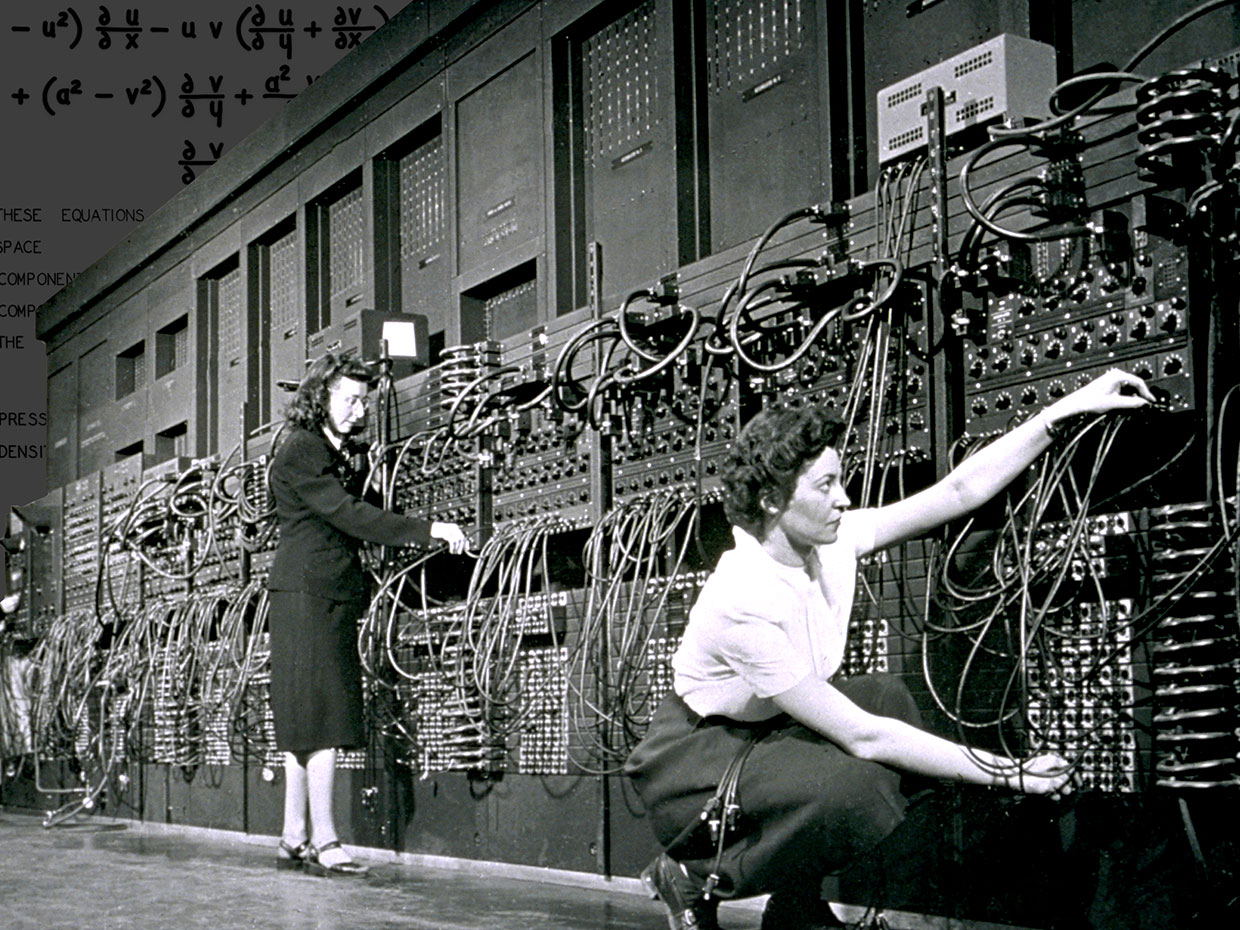
\includegraphics[width=\linewidth,height=5.4cm,keepaspectratio]{figures/p01/eniac.jpg}
\end{columns}
\end{frame}


\begin{frame}{Dôležitý historický problém: ako meniť funkciu stroja?}

\vspace{0.15cm}

\centering

\begin{tikzpicture}[
    stage/.style={
        draw=MainBlue,
        rounded corners=3pt,
        text width=3.25cm,
        minimum height=3.15cm,
        inner xsep=7pt,
        inner ysep=9pt,
        align=center
    }
]

% ============================================================
% PEVNÉ ZAPOJENIE
% ============================================================
\node[
    stage,
    fill=TUKEgray
] (wired) at (0,0)
{%
    {\large\bfseries Pevné zapojenie}

    \vspace{0.35cm}

    {\small
    Funkcia zariadenia je určená fyzickým zapojením obvodov.
    }

    \vfill

    {\color{MainBlue}\small\bfseries
    Zmena = prestavba hardvéru
    }
};

% ============================================================
% PREPÍNAČE A KÁBLE
% ============================================================
\node[
    stage,
    fill=LightBlue
] (panel) at (4.45,0)
{%
    {\large\bfseries Prepínače a káble}

    \vspace{0.35cm}

    {\small
    Funkcia stroja sa mení nastavením prepínačov a prepojením vodičov.
    }

    \vfill

    {\color{MainBlue}\small\bfseries
    Zmena = nové prepojenie
    }
};

% ============================================================
% PROGRAM V PAMÄTI
% ============================================================
\node[
    stage,
    fill=MainBlue,
    text=white
] (program) at (8.90,0)
{%
    {\large\bfseries Program v pamäti}

    \vspace{0.35cm}

    {\small
    Funkciu stroja určujú inštrukcie uložené v pamäti.
    }

    \vfill

    {\color{white}\small\bfseries
    Zmena = nový program
    }
};

% ============================================================
% ŠÍPKY
% ============================================================
\draw[
    ->,
    MainBlue,
    line width=1.1pt
] (wired.east) -- (panel.west);

\draw[
    ->,
    MainBlue,
    line width=1.1pt
] (panel.east) -- (program.west);

\end{tikzpicture}

% \vspace{0.05cm}

\BlueBox{
    \faIcon[regular]{lightbulb}\hspace{0.6em}Kľúčový posun
}{
    \parbox[c][1.25cm][c]{\linewidth}{
        Zavedením programu uloženého v pamäti sa oddelila funkcia stroja
        od jeho fyzického zapojenia. Správanie systému bolo možné meniť
        úpravou programu bez prestavby hardvéru.
    }
}

\end{frame}

\begin{frame}{Tranzistor: základ dnešnej číslicovej techniky}
\begin{columns}[T,onlytextwidth]
\column{0.47\textwidth}
\begin{itemize}
  \item 1947: tranzistor ako polovodičový spínací a zosilňovací prvok.
  \item Oproti elektrónkam priniesol menšie rozmery, nižšiu spotrebu a vyššiu spoľahlivosť.
  \item Umožnil vytvoriť integrované obvody a neskôr mikroprocesory.
\end{itemize}
\begin{alertblock}{Pre študenta}
Každý bit v registri mikrokontroléra je nakoniec realizovaný fyzikálnou štruktúrou z tranzistorov.
\end{alertblock}
\column{0.48\textwidth}
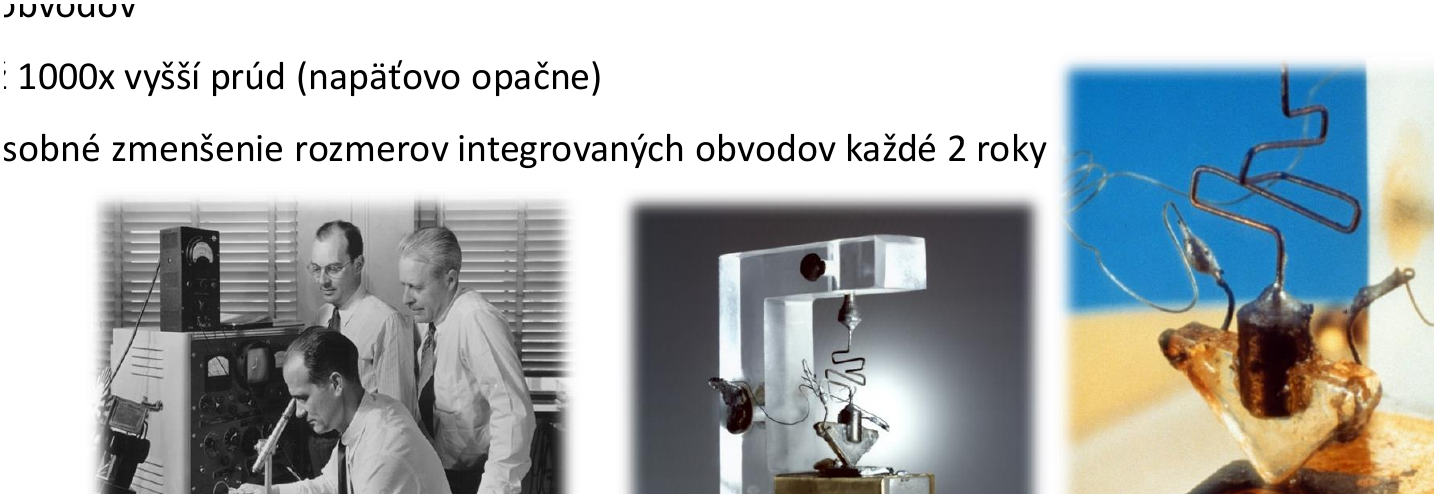
\includegraphics[width=\linewidth,height=4.8cm,keepaspectratio]{transistor_photos.png}
\end{columns}
\end{frame}

\begin{frame}{Integrovaný obvod: logika sa zmenšuje a zlacňuje}
\begin{columns}[T,onlytextwidth]
\column{0.52\textwidth}
\begin{itemize}
  \item Integrácia znamená, že viaceré tranzistory a vodiče sú vytvorené na jednom čipe.
  \item Čím viac logiky je na čipe, tým menej externých spojov a tým vyššia spoľahlivosť.
  \item Základná otázka sa zmenila: koľko funkcie dokážeme dať do jedného obvodu?
\end{itemize}
\column{0.43\textwidth}
\begin{tikzpicture}[x=1cm,y=1cm,scale=0.74,transform shape]
\node[draw=MainBlue,fill=TUKEgray,rounded corners=2pt,minimum width=3.0cm,minimum height=0.9cm] (g1) at (0,2.7) {hradlá};
\node[draw=MainBlue,fill=TUKEgray,rounded corners=2pt,minimum width=3.0cm,minimum height=0.9cm] (g2) at (0,1.5) {registre};
\node[draw=MainBlue,fill=TUKEgray,rounded corners=2pt,minimum width=3.0cm,minimum height=0.9cm] (g3) at (0,0.3) {radič};
\node[draw=MainBlue,fill=MainBlue,text=white,rounded corners=2pt,minimum width=3.0cm,minimum height=3.3cm,align=center] (chip) at (4.4,1.5) {integrovaný\\obvod};
\draw[->,MainBlue,line width=1pt] (g1) -- (chip.west);
\draw[->,MainBlue,line width=1pt] (g2) -- (chip.west);
\draw[->,MainBlue,line width=1pt] (g3) -- (chip.west);
\end{tikzpicture}
\end{columns}
\end{frame}

\begin{frame}{Moorov zákon: prečo sa výpočtová technika tak zrýchlila}
\begin{columns}[T,onlytextwidth]
\column{0.43\textwidth}
\begin{itemize}
  \item Rast počtu tranzistorov umožnil vyšší výkon a nové funkcie.
  \item V mikroprocesoroch viedol k zložitejším CPU a väčším pamätiam.
  \item V embedded systémoch však nie je cieľom iba výkon: dôležitá je cena, spotreba, spoľahlivosť a periférie.
\end{itemize}
\column{0.52\textwidth}
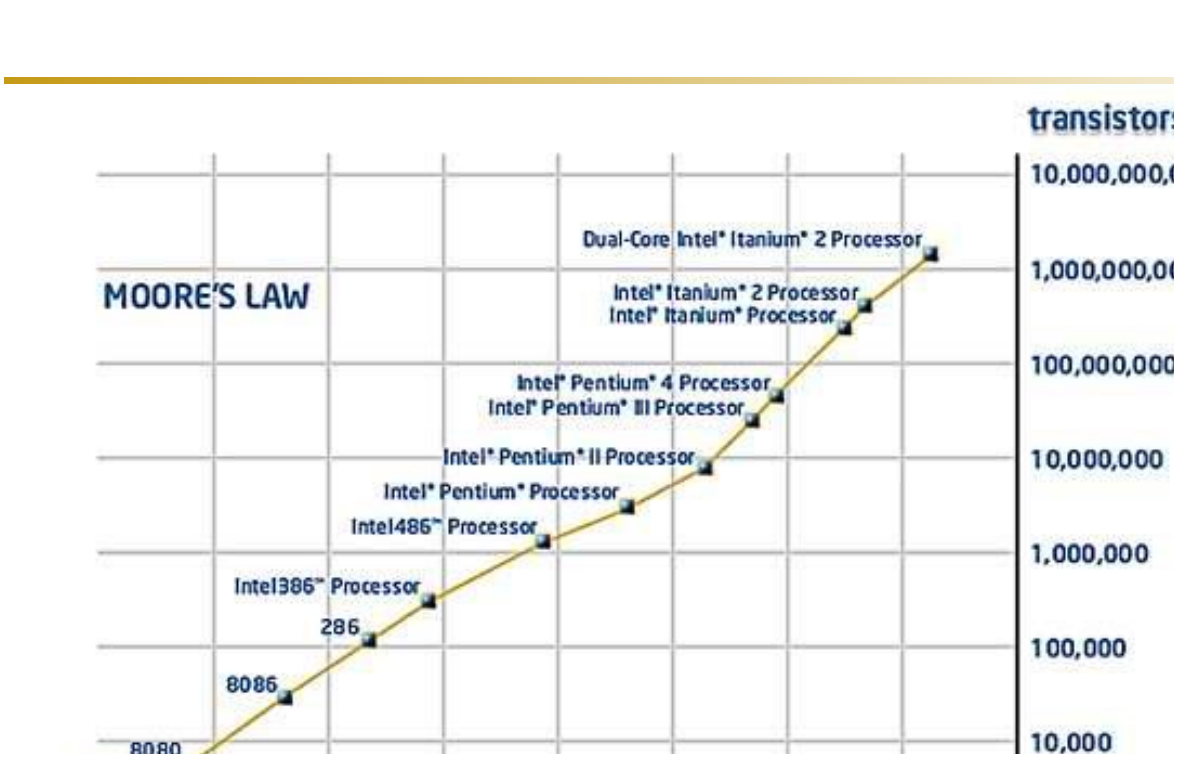
\includegraphics[width=\linewidth,height=5.1cm,keepaspectratio]{moore_graph.png}
\end{columns}
\end{frame}

\begin{frame}{Intel 4004: CPU na jednom čipe}
\begin{columns}[T,onlytextwidth]
\column{0.54\textwidth}
\begin{itemize}
  \item 1971: komerčný 4-bitový mikroprocesor.
  \item Približne 2300 tranzistorov, 16-pinové púzdro.
  \item Vznikol v kontexte kalkulačiek firmy Busicom.
  \item Dôležitý nie je iba výkon, ale nový princíp: procesor ako samostatný integrovaný obvod.
\end{itemize}
\column{0.41\textwidth}
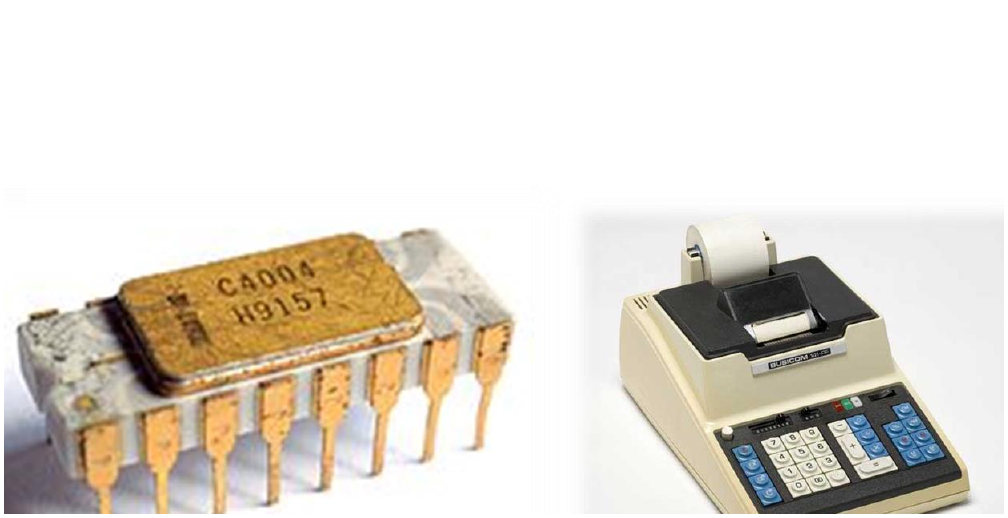
\includegraphics[width=\linewidth,height=4.7cm,keepaspectratio]{intel4004_photos.png}
\end{columns}
\end{frame}

\begin{frame}{Intel 8008: 8-bitové spracovanie dát}
\begin{columns}[T,onlytextwidth]
\column{0.60\textwidth}
\begin{itemize}
  \item 1972: 8-bitový mikroprocesor.
  \item Prechod na 8 bitov uľahčil prácu so znakmi, bajtmi a všeobecnejšími dátami.
  \item Vyžadoval však externé obvody: pamäte, vstupno-výstupné rozhrania a podpornú logiku.
  \item Ešte stále nejde o mikrokontrolér, ale o CPU, okolo ktorého treba postaviť systém.
\end{itemize}
\column{0.34\textwidth}
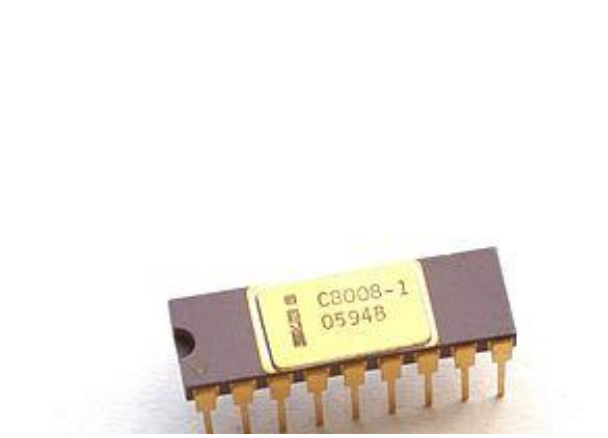
\includegraphics[width=\linewidth,height=4.8cm,keepaspectratio]{intel8008_chip.png}
\end{columns}
\end{frame}

\begin{frame}{Intel 8080: mikroprocesor ako základ riadiaceho systému}
\begin{columns}[T,onlytextwidth]
\column{0.55\textwidth}
\begin{itemize}
  \item 1974: výrazne výkonnejší 8-bitový mikroprocesor.
  \item Používal sa v skorých mikropočítačoch a riadiacich aplikáciách.
  \item Ukázal, že mikroprocesor môže byť centrom všeobecného programovateľného systému.
  \item Pre embedded aplikácie však stále ostával problém veľkosti a počtu externých obvodov.
\end{itemize}
\column{0.40\textwidth}
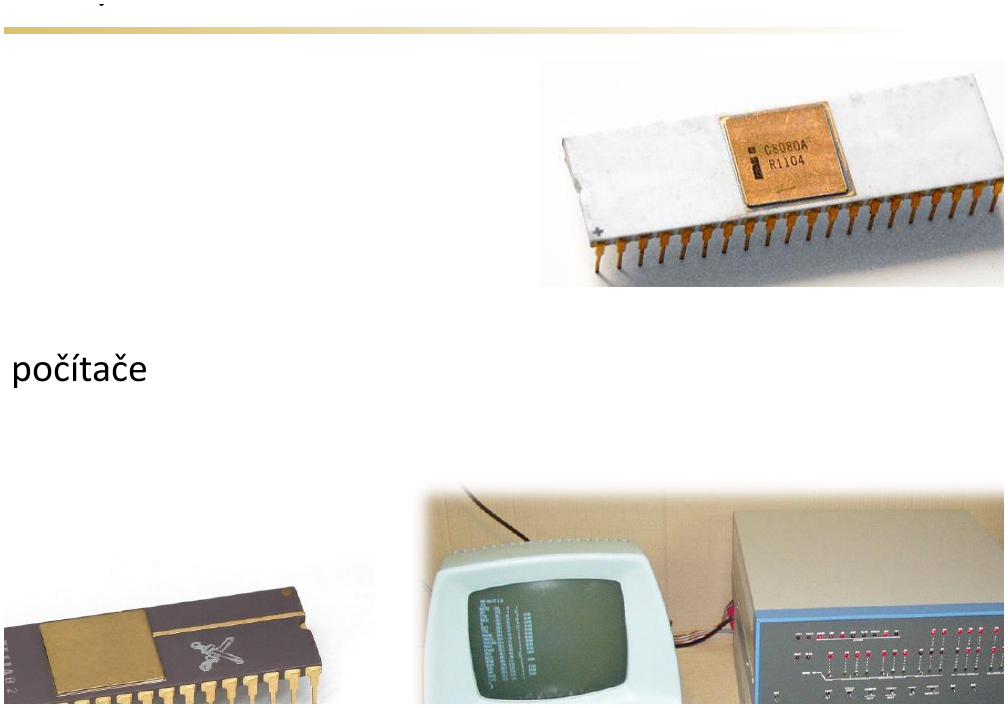
\includegraphics[width=\linewidth,height=5.1cm,keepaspectratio]{intel8080_collage.png}
\end{columns}
\end{frame}

\begin{frame}{Z mikroprocesorového systému k mikrokontroléru}
\begin{center}
\begin{tikzpicture}[x=1cm,y=1cm]
\node[draw=MainBlue,fill=LightBlue,rounded corners=2pt,minimum width=2.5cm,minimum height=0.85cm] (cpu) at (0,2.3) {CPU};
\node[draw=MainBlue,fill=TUKEgray,rounded corners=2pt,minimum width=2.5cm,minimum height=0.85cm] (rom) at (3.2,3.2) {ROM / Flash};
\node[draw=MainBlue,fill=TUKEgray,rounded corners=2pt,minimum width=2.5cm,minimum height=0.85cm] (ram) at (3.2,2.0) {RAM};
\node[draw=MainBlue,fill=TUKEgray,rounded corners=2pt,minimum width=2.5cm,minimum height=0.85cm] (io) at (3.2,0.8) {I/O};
\node[draw=MainBlue,fill=MainBlue,text=white,rounded corners=2pt,minimum width=3.1cm,minimum height=3.0cm,align=center] (mcu) at (8.8,2.0) {CPU\\pamäť\\I/O\\periférie};
\draw[<->,MainBlue,line width=1pt] (cpu) -- (rom);
\draw[<->,MainBlue,line width=1pt] (cpu) -- (ram);
\draw[<->,MainBlue,line width=1pt] (cpu) -- (io);
\draw[->,MainBlue,line width=1.2pt] (5.1,2.0) -- node[above]{integrácia} (7.1,2.0);
\node[font=\small,align=center,text width=4.1cm] at (1.6,0.15) {mikroprocesorový systém z viacerých obvodov};
\node[font=\small,align=center,text width=4.0cm] at (8.8,0.15) {mikrokontrolér ako systém na jednom čipe};
\end{tikzpicture}
\end{center}
\end{frame}

\begin{frame}{TMS1000: CPU, pamäť a I/O na jednom čipe}
\begin{columns}[T,onlytextwidth]
\column{0.52\textwidth}
\begin{itemize}
  \item 1974: rodina mikrokontrolérov Texas Instruments TMS1000.
  \item 4-bitové jadro, ROM, RAM a vstupno-výstupné linky v jednom obvode.
  \item Vhodné pre lacné riadenie kalkulačiek, spotrebnej techniky a jednoduchých zariadení.
  \item Zlomová myšlienka: celý riadiaci systém môže byť integrovaný na jednom čipe.
\end{itemize}
\column{0.43\textwidth}
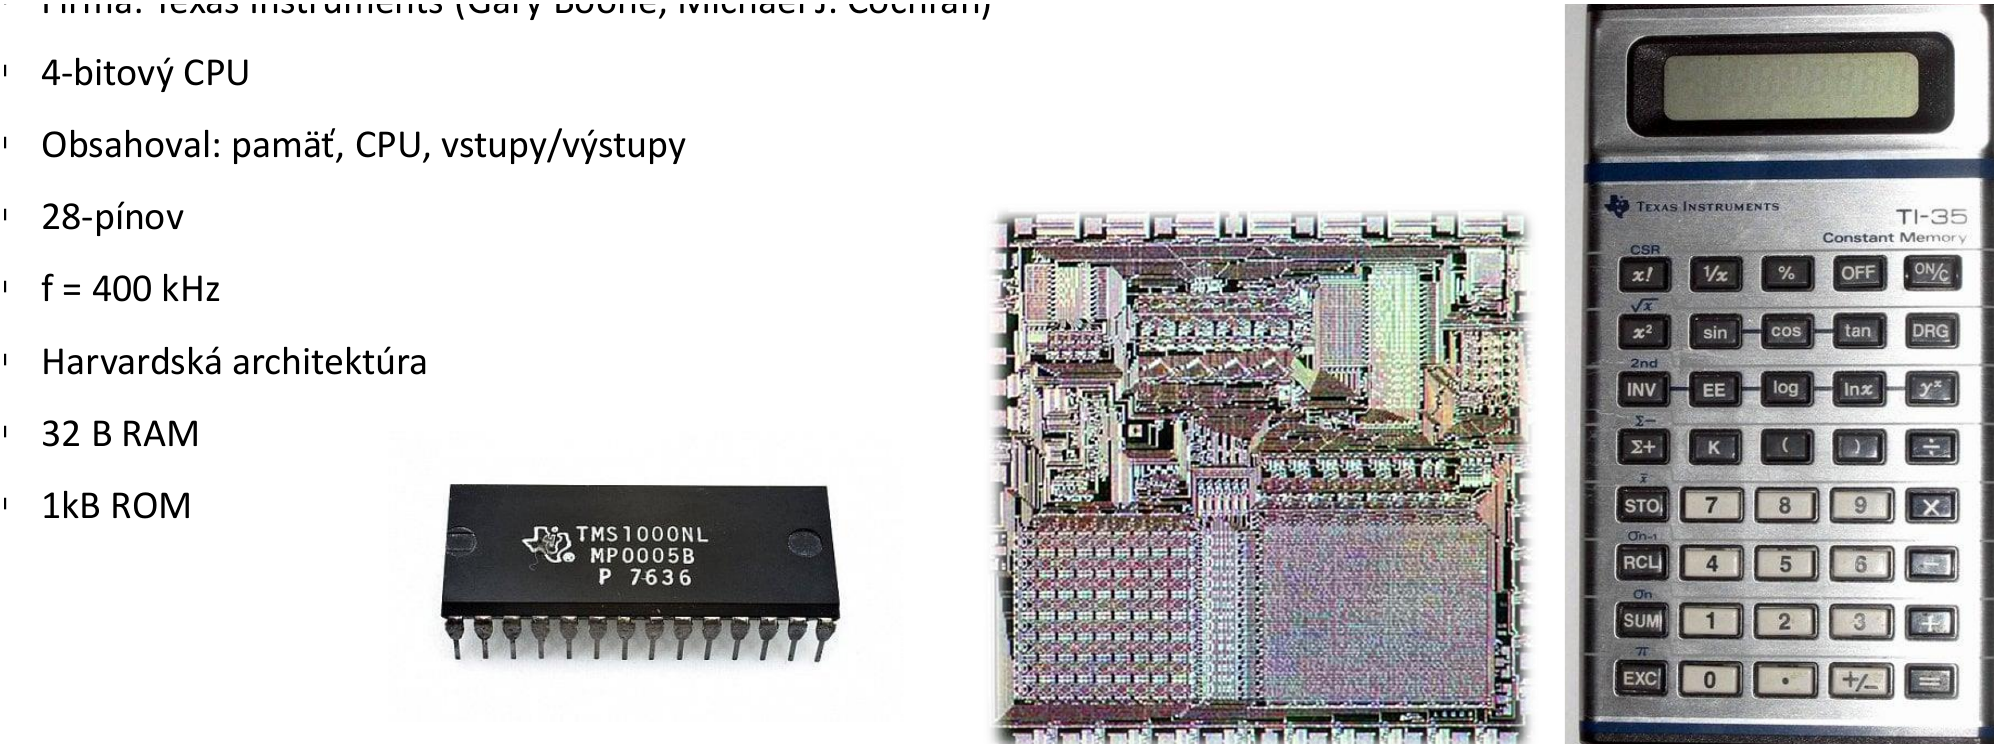
\includegraphics[width=\linewidth,height=5.1cm,keepaspectratio]{tms1000_collage.png}
\end{columns}
\end{frame}

\begin{frame}{Intel 8086: začiatok línie x86}
\begin{columns}[T,onlytextwidth]
\column{0.50\textwidth}
\begin{itemize}
  \item 1978: 16-bitový mikroprocesor.
  \item Dôležitý pre osobné počítače a neskorší vývoj architektúry x86.
  \item Ukazuje inú vetvu vývoja: všeobecné počítače smerovali k rastu výkonu, pamäte a operačným systémom.
  \item Mikrokontroléry smerovali k integrácii, nízkej cene a priamej práci s okolím.
\end{itemize}
\column{0.45\textwidth}
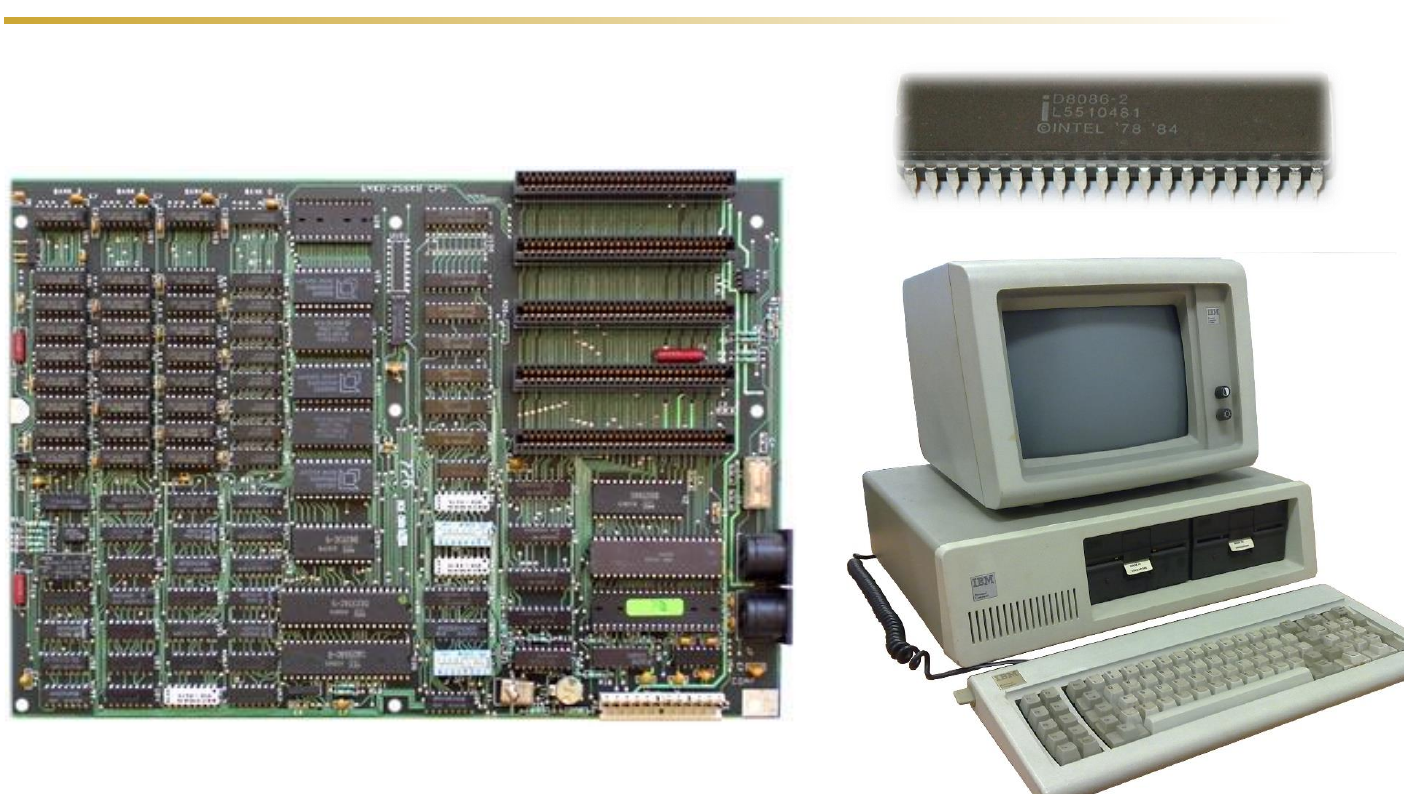
\includegraphics[width=\linewidth,height=5.1cm,keepaspectratio]{intel8086_collage.png}
\end{columns}
\end{frame}

\begin{frame}{Ďalšie míľniky: rozvetvenie vývoja}
\scriptsize
\begin{tabular}{p{0.14\textwidth}p{0.72\textwidth}}
\toprule
Rok & Význam pre mikroprocesorovú a embedded techniku \\
\midrule
1979 & Motorola 68000, Zilog Z8000 - výkonnejšie 16/32-bitové mikroprocesory \\
1980 & Intel 8051 - mimoriadne vplyvná 8-bitová mikrokontrolérová architektúra \\
1983 & TMS32010 - nástup digitálnych signálových procesorov DSP \\
1985 & Intel 80386 - 32-bitová x86 etapa \\
1986 & ARM - RISC architektúra s dôrazom na efektivitu \\
1990s & rozšírenie mikrokontrolérov v automobiloch, spotrebičoch a priemysle \\
2000s & masové embedded systémy, senzory, komunikácia, nízka spotreba \\
2010s+ & IoT, bezpečnosť, viacjadrové MCU, edge AI, hardvérová kryptografia \\
\bottomrule
\end{tabular}
\end{frame}

\begin{frame}{Intel 8051: klasická mikrokontrolérová škola}
\begin{itemize}
  \item 8051 je historicky veľmi významná 8-bitová mikrokontrolérová architektúra.
  \item Typická myšlienka: CPU, pamäť, porty, časovače a sériová komunikácia v jednom systéme.
  \item Mnohé princípy práce s registrami, portmi, prerušením a časovačmi sú podobné aj v AVR.
  \item Preto sa v embedded výučbe často nekladie dôraz na jednu značku čipu, ale na princíp periférií.
\end{itemize}
\begin{alertblock}{Poučenie}
Keď pochopíte jeden mikrokontrolér na úrovni registrov, ľahšie prejdete na ďalší.
\end{alertblock}
\end{frame}

\begin{frame}{ARM: RISC architektúra a nízka spotreba}
\begin{columns}[T,onlytextwidth]
\column{0.55\textwidth}
\begin{itemize}
  \item ARM ukazuje smer k výkonným, ale energeticky efektívnym embedded systémom.
  \item V praxi sa používa od jednoduchých mikrokontrolérov až po aplikačné procesory v mobilných zariadeniach.
  \item Dnešný embedded svet zahŕňa 8-bitové, 16-bitové aj 32-bitové architektúry.
\end{itemize}
\column{0.40\textwidth}
\BlueBox{Prečo teda AVR?}{
AVR je dostatočne jednoduchý na výučbu základov, ale pritom obsahuje reálne periférie používané v embedded praxi: GPIO, časovače, ADC, USART, SPI, TWI.
}
\end{columns}
\end{frame}

\begin{frame}{AVR: vhodná architektúra na výučbu registrov}
\begin{itemize}
  \item 8-bitové AVR mikrokontroléry majú prehľadnú architektúru a dobrú dokumentáciu.
  \item Majú oddelenú pamäť programu a dát, 32 všeobecných registrov a hardvérové periférie.
  \item Sú dostatočne jednoduché na pochopenie, ale nie sú didaktickou hračkou.
  \item ATmega328P je prakticky dostupný na doske Arduino UNO R3, čo znižuje problémy so zapojením.
\end{itemize}
\end{frame}

\begin{frame}{Historický záver}
\begin{center}
\begin{tikzpicture}[x=1cm,y=1cm]
\node[draw=MainBlue,fill=TUKEgray,rounded corners=2pt,minimum width=2.65cm,minimum height=0.8cm,align=center] (a) at (0,2.4) {\textbf{relé}\\\scriptsize pevné zapojenie};
\node[draw=MainBlue,fill=TUKEgray,rounded corners=2pt,minimum width=2.65cm,minimum height=0.8cm,align=center] (b) at (4.0,2.4) {\textbf{elektrónky}\\\scriptsize rýchla logika};
\node[draw=MainBlue,fill=TUKEgray,rounded corners=2pt,minimum width=2.65cm,minimum height=0.8cm,align=center] (c) at (8.0,2.4) {\textbf{tranzistor}\\\scriptsize miniaturizácia};
\node[draw=MainBlue,fill=LightBlue,rounded corners=2pt,minimum width=2.65cm,minimum height=0.8cm,align=center] (d) at (0,0.75) {\textbf{IC}\\\scriptsize integrácia};
\node[draw=MainBlue,fill=LightBlue,rounded corners=2pt,minimum width=2.65cm,minimum height=0.8cm,align=center] (e) at (4.0,0.75) {\textbf{CPU}\\\scriptsize mikroprocesor};
\node[draw=MainBlue,fill=MainBlue!18,rounded corners=2pt,minimum width=2.65cm,minimum height=0.8cm,align=center] (f) at (8.0,0.75) {\textbf{MCU}\\\scriptsize systém na čipe};
\draw[->,MainBlue,line width=1pt] (a) -- (b);
\draw[->,MainBlue,line width=1pt] (b) -- (c);
\draw[->,MainBlue,line width=1pt] (c.south) .. controls (8,-0.15) and (0,1.75) .. (d.north);
\draw[->,MainBlue,line width=1pt] (d) -- (e);
\draw[->,MainBlue,line width=1pt] (e) -- (f);
\end{tikzpicture}
\end{center}
\vspace{0.2cm}
\BlueBox{Zmysel tejto línie}{Mikrokontrolér vznikol, keď sa do jedného lacného a spoľahlivého obvodu integrovali výpočet, pamäť a priame rozhranie s okolím.}
\end{frame}

\SectionFrame{2. Základné pojmy}{Pojmy, ktoré budeme používať pri práci s datasheetom a registrami.}

\begin{frame}{Mikroprocesor verzus mikrokontrolér}
\small
\begin{tabular}{p{0.27\textwidth}p{0.31\textwidth}p{0.33\textwidth}}
\toprule
Vlastnosť & Mikroprocesor & Mikrokontrolér \\
\midrule
Hlavná úloha & všeobecné výpočty & riadenie konkrétneho zariadenia \\
Pamäť & často externá & typicky integrovaná \\
Periférie & externé obvody & GPIO, časovače, ADC, komunikácie \\
Operačný systém & často áno & často bez OS \\
Typické kritériá & výkon, pamäť, OS & cena, spotreba, real-time, spoľahlivosť \\
Príklad & PC procesor & ATmega328P, STM32, PIC, ESP32 \\
\bottomrule
\end{tabular}
\end{frame}

\begin{frame}{Čo je vo vnútri mikrokontroléra}
\begin{columns}[T,onlytextwidth]
\column{0.48\textwidth}
\begin{itemize}
  \item \textbf{CPU}: vykonáva inštrukcie.
  \item \textbf{Flash}: programová pamäť.
  \item \textbf{SRAM}: premenné a zásobník.
  \item \textbf{EEPROM}: trvalo uložené konfiguračné údaje.
  \item \textbf{Periférie}: porty, časovače, ADC, komunikácie.
\end{itemize}
\column{0.47\textwidth}
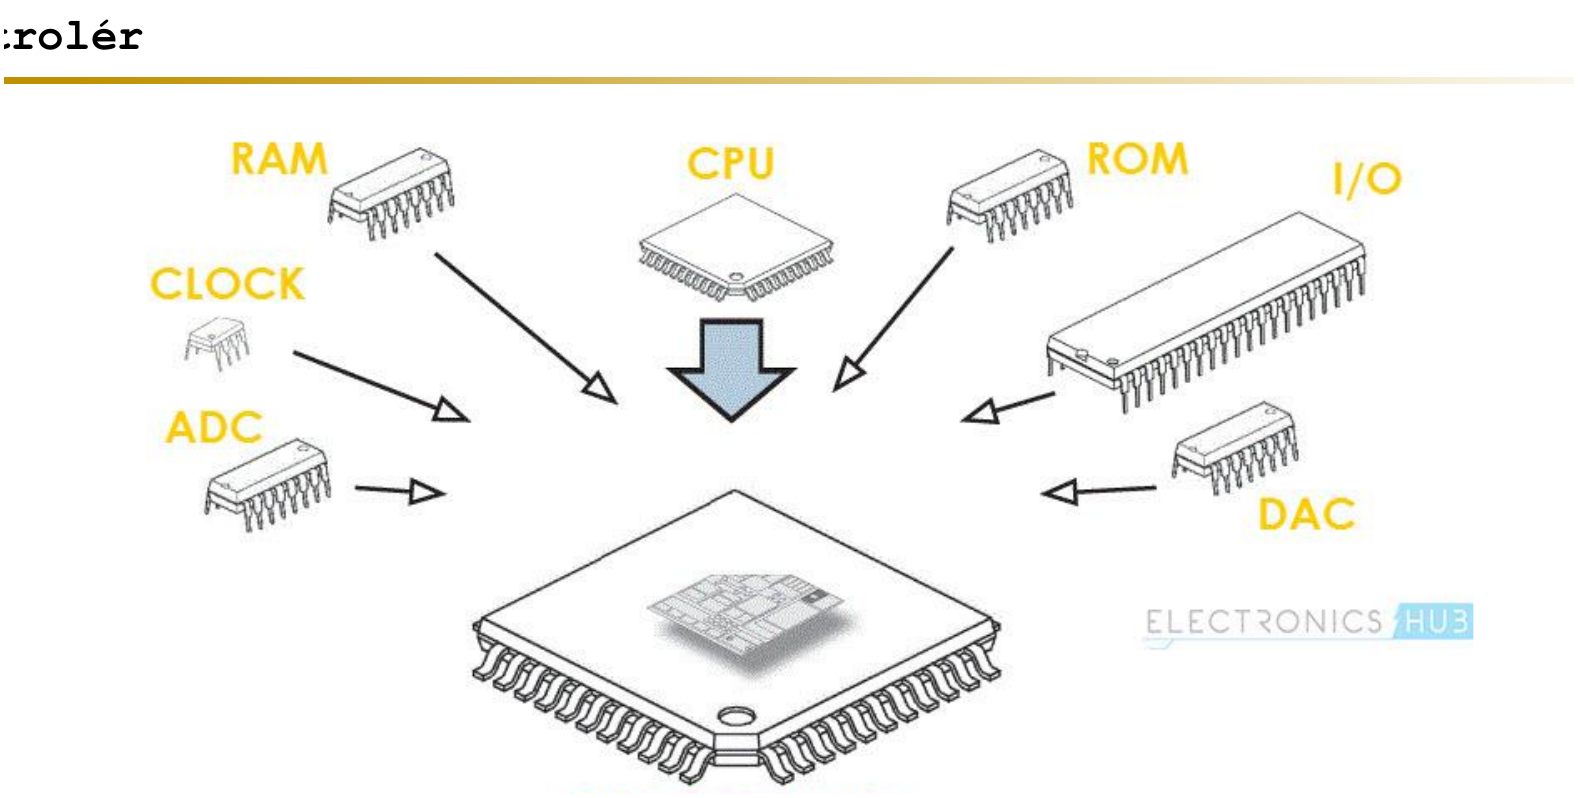
\includegraphics[width=\linewidth,height=5.0cm,keepaspectratio]{microcontroller_components.png}
\end{columns}
\end{frame}

\begin{frame}{Základné pojmy procesora}
\begin{columns}[T,onlytextwidth]
\column{0.49\textwidth}
\begin{itemize}
  \item \textbf{Inštrukcia}: elementárny príkaz CPU.
  \item \textbf{Inštrukčný súbor}: dostupné príkazy procesora.
  \item \textbf{ALU}: aritmeticko-logická jednotka.
  \item \textbf{Register}: rýchla pamäťová bunka v CPU alebo periférii.
\end{itemize}
\column{0.47\textwidth}
\begin{itemize}
  \item \textbf{PC}: programový čítač.
  \item \textbf{SP}: ukazovateľ zásobníka.
  \item \textbf{SREG}: stavový register s príznakmi.
  \item \textbf{Zásobník}: dočasné dáta, návratové adresy, obsluha prerušení.
\end{itemize}
\end{columns}
\end{frame}

\begin{frame}{Zbernice: dáta, adresy a riadenie}
\begin{center}
\begin{tikzpicture}[x=1cm,y=1cm]
\node[draw=MainBlue,fill=MainBlue,text=white,rounded corners=2pt,minimum width=2.8cm,minimum height=0.9cm] (cpu) at (0,1.8) {CPU};
\node[draw=MainBlue,fill=LightBlue,rounded corners=2pt,minimum width=2.8cm,minimum height=0.9cm] (mem) at (5.2,2.7) {pamäť};
\node[draw=MainBlue,fill=LightBlue,rounded corners=2pt,minimum width=2.8cm,minimum height=0.9cm] (io) at (5.2,0.9) {periféria};
\draw[<->,MainBlue,line width=1.1pt] (cpu) -- node[above,sloped]{dátová zbernica} (mem);
\draw[->,MainBlue,line width=1.1pt] (cpu) -- node[below,sloped]{adresná zbernica} (mem);
\draw[<->,MainBlue,line width=1.1pt] (cpu) -- node[below,sloped]{riadiace signály} (io);
\end{tikzpicture}
\end{center}
\begin{itemize}
  \item Dátová zbernica prenáša hodnoty.
  \item Adresná zbernica určuje, s ktorou bunkou alebo registrom sa pracuje.
  \item Riadiace signály určujú čítanie, zápis, prerušenie alebo stav periférie.
\end{itemize}
\end{frame}

\begin{frame}{Von Neumannova a Harvardská architektúra}
\begin{columns}[T,onlytextwidth]
\column{0.48\textwidth}
\BlueBox{Von Neumann}{
\begin{itemize}
  \item spoločná pamäť pre program aj dáta,
  \item jednoduchší model,
  \item možné úzke hrdlo pri prístupe do pamäte.
\end{itemize}}
\column{0.48\textwidth}
\BlueBox{Harvard}{
\begin{itemize}
  \item oddelená pamäť programu a dát,
  \item paralelnejší prístup,
  \item typické pre mnohé mikrokontroléry vrátane AVR.
\end{itemize}}
\end{columns}
\end{frame}

\begin{frame}{CISC, RISC a praktický význam pre C program}
\begin{itemize}
  \item \textbf{CISC}: rozsiahly súbor inštrukcií, často zložitejšie inštrukcie.
  \item \textbf{RISC}: jednoduchšie inštrukcie, viac registrov, dôraz na rýchle vykonávanie.
  \item AVR je 8-bitová RISC architektúra s 32 všeobecnými pracovnými registrami.
  \item Aj keď budeme písať v C, prekladač generuje konkrétne inštrukcie a prístupy do registrov.
\end{itemize}
\begin{alertblock}{Dôležité}
C kód v embedded systéme nie je izolovaný od hardvéru. Každý prístup do registra môže zmeniť správanie periférie.
\end{alertblock}
\end{frame}

\begin{frame}{Hodinový cyklus, strojový cyklus, real-time}
\begin{columns}[T,onlytextwidth]
\column{0.55\textwidth}
\begin{itemize}
  \item Hodinový signál určuje základný rytmus procesora.
  \item ATmega328P na Arduino UNO R3 je typicky taktovaný na 16 MHz.
  \item Nie každá inštrukcia znamená jeden užitočný regulačný výpočet.
  \item V embedded systéme musíme rozumieť časovaniu: oneskorenie, latencia prerušenia, perióda vzorkovania.
\end{itemize}
\column{0.40\textwidth}
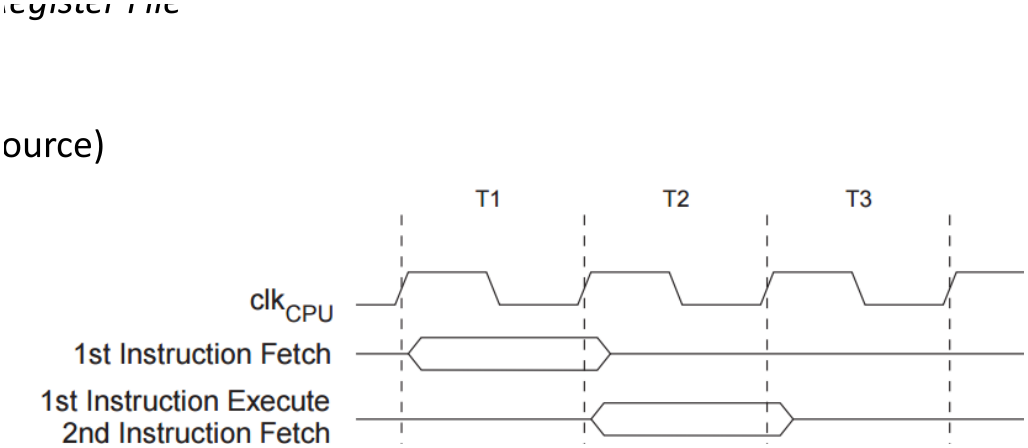
\includegraphics[width=\linewidth,height=4.2cm,keepaspectratio]{pipeline.png}
\end{columns}
\end{frame}

\SectionFrame{3. Platforma predmetu}{Arduino UNO R3 ako doska, ATmega328P ako mikrokontrolér, bare-metal AVR C ako spôsob programovania.}

\begin{frame}{Prečo Arduino UNO R3, keď nechceme Arduino framework}
\begin{itemize}
  \item UNO R3 rieši praktické veci: napájanie, USB, reset, hodinový zdroj, bootloader a konektory.
  \item Tým sa zníži počet chýb spôsobených breadboardom a vodičmi.
  \item Študent sa môže sústrediť na mikrokontrolér, registre a periférie.
  \item Doska je iba nosič ATmega328P, nie dôvod používať \texttt{digitalWrite()}.
\end{itemize}
\begin{alertblock}{Pravidlo predmetu}
Hardvér Arduino UNO R3 áno. Arduino framework nie.
\end{alertblock}
\end{frame}

\begin{frame}{ATmega328P: základné parametre}
\small
\begin{tabular}{p{0.34\textwidth}p{0.53\textwidth}}
\toprule
Parameter & Význam pre predmet \\
\midrule
8-bit AVR RISC & jednoduchá a čitateľná architektúra \\
32 kB Flash & program uložený v mikrokontroléri \\
2 kB SRAM & premenné, zásobník, buffre \\
1 kB EEPROM & trvalé konfiguračné dáta \\
23 GPIO liniek & digitálne vstupy a výstupy \\
3 časovače/čítače & časovanie, PWM, meranie impulzov \\
10-bit ADC & meranie analógových snímačov \\
USART, SPI, TWI & sériová komunikácia s okolím \\
Watchdog & zotavenie z poruchového stavu \\
\bottomrule
\end{tabular}
\end{frame}

\begin{frame}{ATmega328P ako blokový systém}
\begin{columns}[T,onlytextwidth]
\column{0.48\textwidth}
\begin{itemize}
  \item Jadrom je AVR CPU s registrami a ALU.
  \item Periférie sú pripojené cez vnútorné zbernice.
  \item Každá periféria má riadiace, stavové a dátové registre.
  \item Program pracuje s hardvérom práve cez tieto registre.
\end{itemize}
\column{0.47\textwidth}
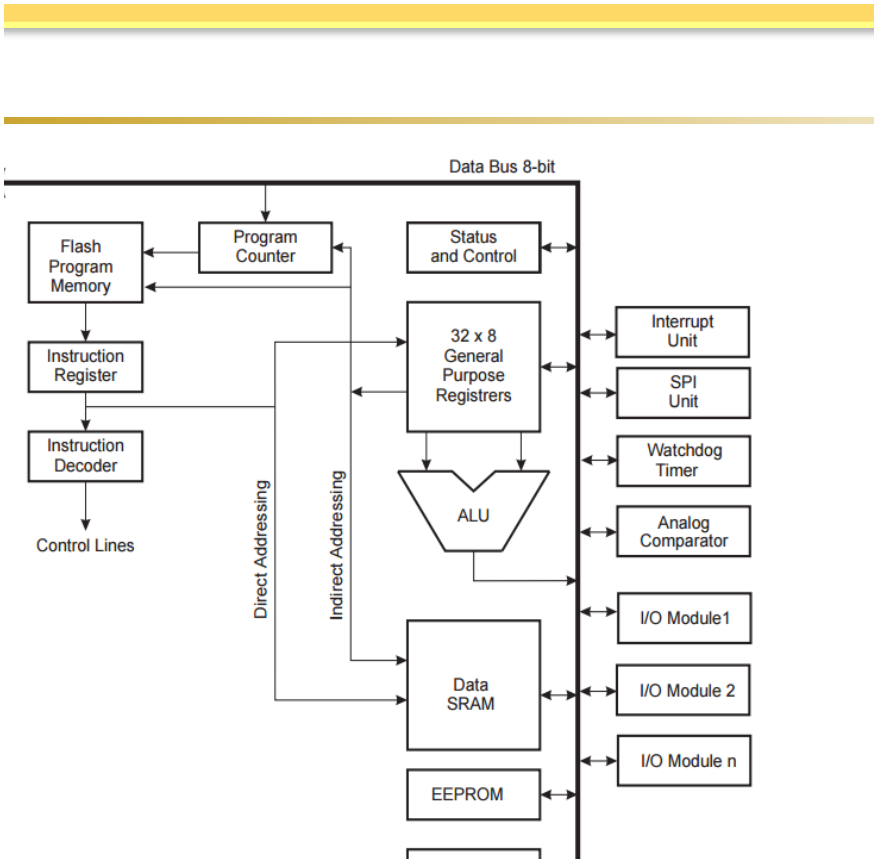
\includegraphics[width=\linewidth,height=5.2cm,keepaspectratio]{atmega328_block.png}
\end{columns}
\end{frame}

\begin{frame}{Register ako rozhranie medzi programom a hardvérom}
\begin{columns}[T,onlytextwidth]
\column{0.46\textwidth}
\begin{itemize}
  \item Register nie je obyčajná premenná v RAM.
  \item Bit v registri môže povoliť prerušenie, nastaviť režim časovača alebo zmeniť smer pinu.
  \item Datasheet presne definuje význam každého bitu.
\end{itemize}
\column{0.49\textwidth}
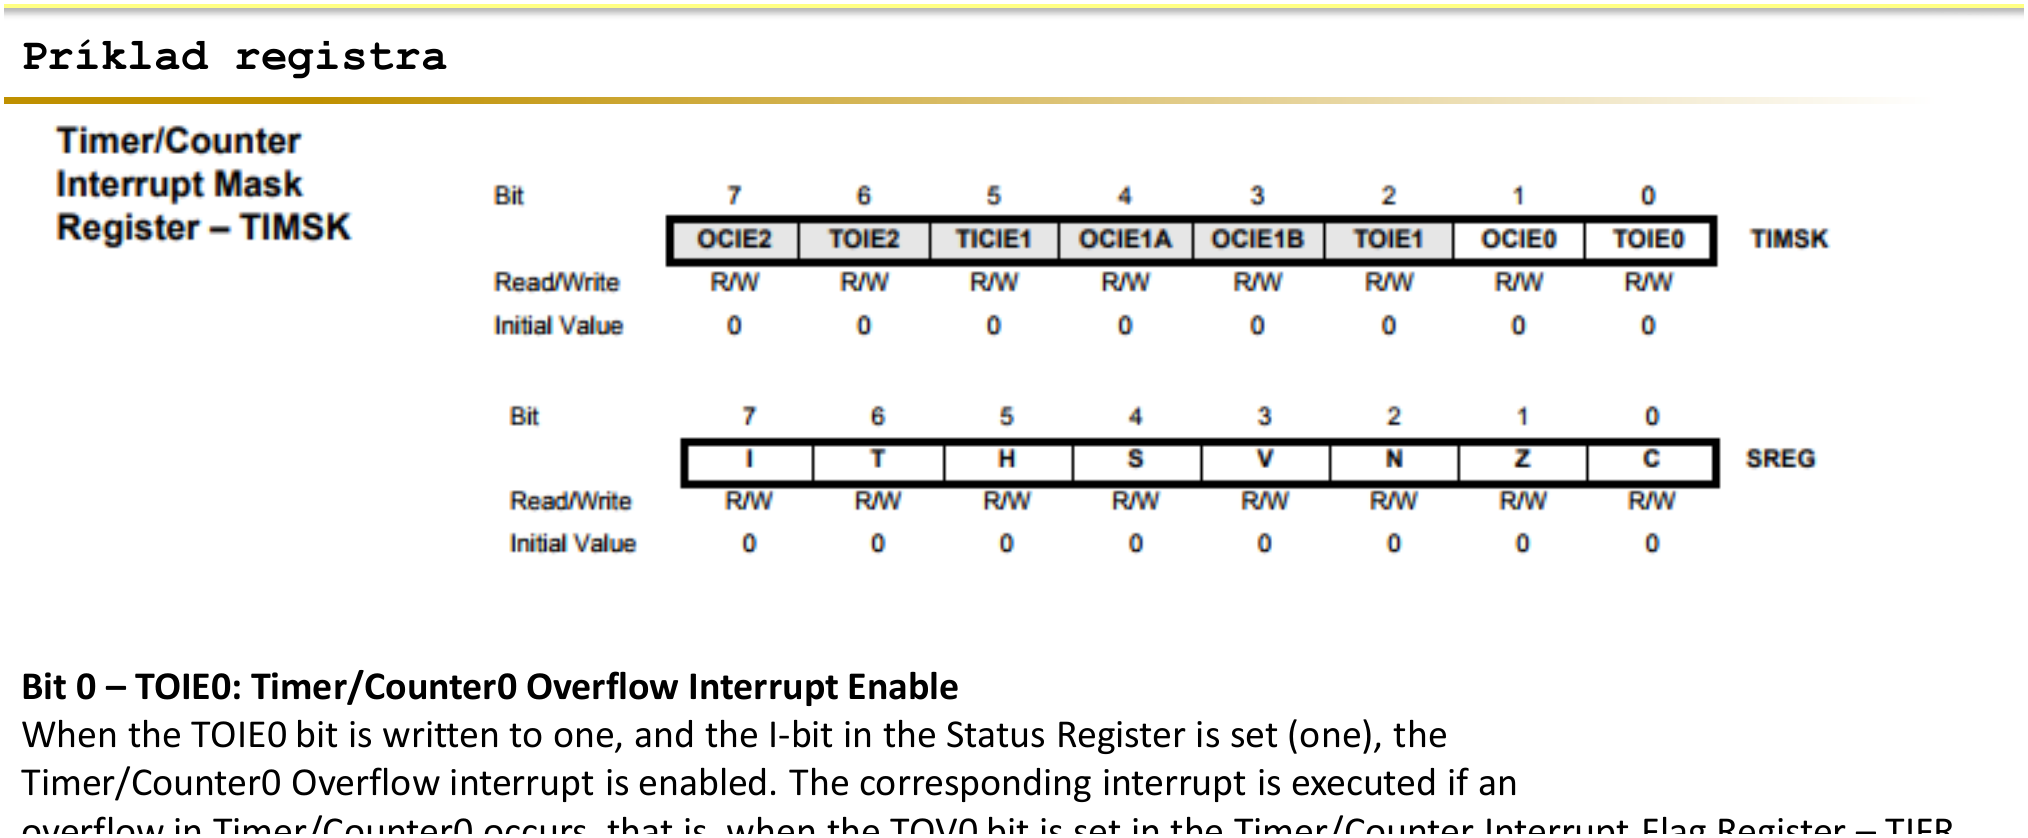
\includegraphics[width=\linewidth,height=4.8cm,keepaspectratio]{register_example.png}
\end{columns}
\end{frame}

\begin{frame}[fragile]{Príklad: zápis do registra portu}
\begin{lstlisting}[style=avrstyle]
DDRB  |= (1 << DDB5);    // PB5 ako vystup
PORTB |= (1 << PORTB5);  // log. 1 na PB5
PORTB &= ~(1 << PORTB5); // log. 0 na PB5
\end{lstlisting}
\vspace{0.1cm}
\begin{itemize}
  \item \texttt{DDRB}: smer pinov portu B,
  \item \texttt{PORTB}: výstupná hodnota alebo pull-up,
  \item \texttt{PINB}: čítanie logického stavu pinov.
\end{itemize}
\begin{alertblock}{Most k ďalšej prednáške}
V druhej prednáške už z týchto troch registrov spravíme LED, tlačidlo a jednoduché digitálne rozhranie.
\end{alertblock}
\end{frame}

\begin{frame}[fragile]{Základný program v tomto predmete}
\begin{lstlisting}[style=avrstyle]
#include <avr/io.h>
#include <avr/interrupt.h>

int main(void)
{
    // konfiguracia registrov periferii

    while (1)
    {
        // hlavna slucka programu
    }

    return 0;
}
\end{lstlisting}
\end{frame}

\begin{frame}{Vývojový reťazec}
\begin{center}
\begin{tikzpicture}[x=1cm,y=1cm]
\node[draw=MainBlue,fill=LightBlue,rounded corners=2pt,minimum width=2.3cm,minimum height=0.85cm] (src) at (0,1.6) {\texttt{main.c}};
\node[draw=MainBlue,fill=LightBlue,rounded corners=2pt,minimum width=2.3cm,minimum height=0.85cm] (gcc) at (3.0,1.6) {AVR-GCC};
\node[draw=MainBlue,fill=LightBlue,rounded corners=2pt,minimum width=2.3cm,minimum height=0.85cm] (hex) at (6.0,1.6) {\texttt{.hex}};
\node[draw=MainBlue,fill=MainBlue,text=white,rounded corners=2pt,minimum width=2.3cm,minimum height=0.85cm] (mcu) at (9.0,1.6) {ATmega328P};
\draw[->,MainBlue,line width=1pt] (src) -- (gcc);
\draw[->,MainBlue,line width=1pt] (gcc) -- (hex);
\draw[->,MainBlue,line width=1pt] (hex) -- node[above]{AVRDUDE} (mcu);
\end{tikzpicture}
\end{center}
\BlueBox{Úloha PlatformIO}{PlatformIO je prostredie, ktoré volá prekladač, linker a nahrávací nástroj. Cieľom predmetu však ostáva porozumenie mikrokontroléru.}
\end{frame}

\begin{frame}[fragile]{Minimálny projekt v PlatformIO}
\begin{lstlisting}[style=avrstyle]
; platformio.ini
[env:uno]
platform = atmelavr
board = uno

build_flags =
    -std=gnu11
    -Wall
    -Wextra
    -Wpedantic
\end{lstlisting}
\begin{alertblock}{Kontrola}
V projekte nesmie byť uvedené \texttt{framework = arduino}. Zdrojový súbor má byť \texttt{main.c}, nie \texttt{main.ino}.
\end{alertblock}
\end{frame}

\begin{frame}{Prvé laboratórne cvičenie}
\begin{itemize}
  \item inštalácia a kontrola VS Code, PlatformIO, AVR toolchainu,
  \item vytvorenie projektu pre dosku \texttt{uno},
  \item kompilácia minimálneho programu,
  \item nahratie pripraveného programu do UNO R3,
  \item orientácia na doske: napájanie, USB, reset, digitálne a analógové piny,
  \item vysvetlenie mapovania Arduino pinov na porty ATmega328P.
\end{itemize}
\end{frame}

\begin{frame}{Ako budeme čítať datasheet}
\begin{columns}[T,onlytextwidth]
\column{0.48\textwidth}
\BlueBox{Postup}{
\begin{enumerate}
  \item nájsť kapitolu periférie,
  \item identifikovať registre,
  \item pochopiť význam bitov,
  \item nastaviť bity maskou,
  \item overiť správanie meraním.
\end{enumerate}}
\column{0.48\textwidth}
\BlueBox{Inžinierska disciplína}{
\begin{itemize}
  \item žiadne slepé kopírovanie kódu,
  \item komentovať rozhodujúce bity,
  \item myslieť na elektrické limity,
  \item uvažovať bezpečný stav zariadenia.
\end{itemize}}
\end{columns}
\end{frame}

\begin{frame}{Prepojenie na druhú prednášku}
\begin{itemize}
  \item Dnes sme vysvetlili, prečo mikrokontrolér vznikol a čo obsahuje.
  \item Nabudúce prejdeme ku konkrétnej periférii: digitálne vstupy a výstupy.
  \item Budeme používať registre \texttt{DDRx}, \texttt{PORTx} a \texttt{PINx}.
  \item Prvé praktické úlohy budú LED, tlačidlo, pull-up rezistor, aktívna nula a bitové masky.
\end{itemize}
\begin{alertblock}{Otázka na prípravu}
Prečo je bezpečnejšie nastaviť iba jeden bit registra maskou než zapísať do celého registra novú hodnotu?
\end{alertblock}
\end{frame}

\begin{frame}{Zhrnutie prednášky}
\begin{itemize}
  \item Vývoj smeroval od pevne zapojenej logiky k programovateľnému riadeniu.
  \item Mikroprocesor integroval CPU na jeden čip, mikrokontrolér integroval celý riadiaci systém.
  \item Embedded systém spája program, elektroniku, snímače, aktuátory a časovanie.
  \item Arduino UNO R3 používame ako hardvérovú dosku s ATmega328P.
  \item Programovať budeme bare-metal AVR C, teda priamo cez registre a datasheet.
\end{itemize}
\end{frame}

\begin{frame}{Použitá a odporúčaná literatúra}
\footnotesize
\begin{itemize}
  \item Microchip Technology: \textit{ATmega328P product page and datasheet}.
  \item Arduino Documentation: \textit{Arduino UNO Rev3}.
  \item Intel: \textit{The First Programmable Microprocessor: The 4004}.
  \item Texas Instruments / historické zdroje k TMS1000 a skorým mikrokontrolérom.
  \item Atmel/Microchip: \textit{AVR Instruction Set Manual}.
  \item Pôvodná prednáška predmetu Mikroprocesorová technika - použité a prepracované historické obrazové materiály.
\end{itemize}
\end{frame}


\TUKEclosingframe{Otázky?}

\end{document}
